%%%%%%%%%%%%%%%%%%%%%%%%%%%%%%%%%%%%%%%%%%%%%%%%%%%%%%%%%%%%%%%%%%%%%%
% DOCUMENTCLASS
%%%%%%%%%%%%%%%%%%%%%%%%%%%%%%%%%%%%%%%%%%%%%%%%%%%%%%%%%%%%%%%%%%%%%%

\documentclass[12pt]{article}

%%%%%%%%%%%%%%%%%%%%%%%%%%%%%%%%%%%%%%%%%%%%%%%%%%%%%%%%%%%%%%%%%%%%%%
% PACKAGES
%%%%%%%%%%%%%%%%%%%%%%%%%%%%%%%%%%%%%%%%%%%%%%%%%%%%%%%%%%%%%%%%%%%%%%

\usepackage{epsfig}
%\usepackage{times}
\usepackage{url}

%%%%%%%%%%%%%%%%%%%%%%%%%%%%%%%%%%%%%%%%%%%%%%%%%%%%%%%%%%%%%%%%%%%%%%
% FORMATTING
%%%%%%%%%%%%%%%%%%%%%%%%%%%%%%%%%%%%%%%%%%%%%%%%%%%%%%%%%%%%%%%%%%%%%%

\textwidth=7.0in
\oddsidemargin=-0.25in
%\evensidemargin=-0.25in
\textheight=9.0in
\topmargin=-0.75in
\columnsep=0.25in

%%%%%%%%%%%%%%%%%%%%%%%%%%%%%%%%%%%%%%%%%%%%%%%%%%%%%%%%%%%%%%%%%%%%%%
% BEGIN DOC
%%%%%%%%%%%%%%%%%%%%%%%%%%%%%%%%%%%%%%%%%%%%%%%%%%%%%%%%%%%%%%%%%%%%%%
\begin{document}
%\baselineskip=11.2pt

\title{ROSS/ROSS.Net: Rensselaer's Optimistic Simulation System\\ User's Guide}

\author{
 Christopher D. Carothers -- RPI CS Faculty  \\[12pt]
 Mark Anderson -- RPI CS PhD Student       \\
 David Bauer -- MITRE                      \\	
 Akintayo Holder -- RPI CS PhD Student     \\
 Justin Lapre -- RPI CS PhD Student        \\
 Shawn Pearce -- Google                    \\
 Garrett Yaun -- Google                    \\[12pt]
                                           \\
 Department of Computer Science \\
 Rensselaer Polytechnic Institute \\
 Troy, NY 12180, U.S.A.\\
 {\em chrisc@cs.rpi.edu}\\ \\
}

\date{\today}
\maketitle

\pagebreak

\tableofcontents

\pagebreak

\section{ROSS}
ROSS is an acronym for Rensselaer's Optimistic Simulation System.  It is a
parallel discrete-event simulator that executes on shared-memory
multiprocessor systems. ROSS is geared for running large-scale simulation
models (i.e., 100K to even 1 million object models).

The synchronization mechanism is based on Time Warp. Time Warp is an
optimistic synchronization mechanism develop by Jefferson and
Sowizral~\cite{jefferson-tr-82,jefferson-toplas-85} used in the
parallelization of discrete-event simulation. The distributed simulator
consists of a collection of {\em logical processes} or LPs, each modeling a
distinct component of the system being modeled, e.g., a server in a queuing
network.  LPs communicate by exchanging timestamped event messages, e.g.,
denoting the arrival of a new job at that server.

The Time Warp mechanism uses a detection-and-recovery protocol to synchronize
the computation.  Any time an LP determines that it has processed events out
of timestamp order, it ``rolls back'' those events, and re-executes them. For
a detailed discussion of Time Warp as well as other parallel simulation
protocols we refer the reader to~\cite{fujimoto-cacm-1990}

ROSS was modeled after a Time Warp simulator called GTW or Georgia Tech Time
Warp\cite{das-wsc-1994}. ROSS helped to demonstrate that Time Warp simulators
can be run efficiently both in terms of speed and memory usage relative to a
high-performance sequential simulator.

To achieve high parallel performance, ROSS uses a technique call Reverse
Computation. Here, the roll back mechanism in the optimistic simulator is
realized not by classic state-saving, but by literally allowing to the
greatest possible extent events to be reverse. Thus, as models are developed
for parallel execution, both the forward and reverse execution code must be
written. Currently, both are done by hand. We are investigating automatic
methods that are able to generate the reverse execution code using only the
forward execution code as input. For more information on ROSS and Reverse
Computation we refer the interested reader to~\cite{carothers-tomacs-1999,
  carothers-pads-2000}. Both of these text are provided as additional reading
in the ROSS distribution.

\subsection{Quick Build}

Copy the following script, call it {\tt ross-get.sh} and run it in
the directory to where you would like the {\tt rossnet} source code
installed along with the {\tt rossnet-build} directory.

\begin{verbatim}
#!/bin/sh

svn co https://subversion.cs.rpi.edu/svn/rossnet

mkdir rossnet-build
cd ross-build

# Edit ARCH to be one of x86_64 for Linux/x86 systems 
#                        bgl for Blue Gene/L
#                        bgp for Blue Gene/P
#                        ppc64 for PowerPC systems
export ARCH=x86_64

# Edit CC to point to the right MPI pre-compiler script
export CC=/usr/local/mpich2-1.2/bin/mpicc

# Make sure you have Cmake install on system.
# Ross/ROSS.Net requires Cmake 2.8
cmake ../rossnet

# Build Ross models and ROSS.Net
make -j 8

# Start MPI Daemon -- delete if not required for your
# version of MPI
mpd &

# Run ROSS.Net

cd ../rossnet/trunk/rnf/kernel
ln -s ../../../../rossnet-build/trunk/rnf/kernel/rn ./rn

# Executes the TCP2 model using Optimistic synchronization
# Make sure you edit the clock rate for your processor speed.
mpirun -np 4 ./rn --scenario=tcp2 --synch=3 --clock-rate=2667000000 --nkp=512 --batch=2 --gvt-interval=64
\end{verbatim}
 

\subsection{Data Structures}
ROSS allows for an application programmer to design an application with the
ROSS API which will simulate some real world event.  The model that we use for
testing and educational purposes is called {\em pcs}, which is short for
``personal communications services''.  PCS simulates PCS/mobile phones calls
being generated at a cell phone tower, and then moved around to other towers
at some later time, and then the phone call ends.  At the end of a phone call,
another call or two may be generated.  At the end of the simulation,
statistics regarding how often calls were blocked (busy) due to limited tower
capacity etc were collected. This details for this model can be found
in~\cite{carothers-pads-1995}. This paper is included with this ROSS
distribution.

ROSS utilizes three main data structures in C.  There is a PE (short for
processor) struct, an LP struct (short for Logical Process) and an event
struct.  It will be necessary to understand these structures if you are going
to complete an application of your own design within ROSS.
 
\subsubsection{Events}
This is the most basic part of the ROSS system.  An event is simply that, an
event that occurs in the system.  The ROSS engine operates on events in what
we call time-stamp order.  So, if we have three events with simulation
timestamps of 5, 10 and 15, then the application developer would expect for
the ROSS engine to process the event with a timestamp of 5 first, then 10
second and finally 15.  Successful applications will first prime the system
with a few events, and then ensure that when events are processed and leave
the system that new events will be created.  So, with this understanding of
events, we need to know what data fields within the struct are available and
important to us, the application designer.

\begin{verbatim}
	/*
        * tw_event:
        *
        * Holds entire event structure, one is created for each and every
        * event in use.  We preallocate tw_message's into tw_event at
        * startup time so that there is no overhead of trying to locate the
        * tw_message storage area.  The tw_message MUST be the last item
        * in the tw_event.
       */

	DEF(struct, tw_event)
	{
\end{verbatim}

These variables are strictly for event processing and are not part of
the API.

\begin{verbatim}
       /*
        * next         -- Next pointer for all queues.
        * prev         -- Used by some queues.
        * up           -- Used by some queues.
        * cancel_next  -- Next event in the cancel queue for the dest_pe.
        * caused_by_me -- Start of event list caused by this event.
        * cause_list   -- List of events caused by the event with its
        *                 caused_by_me pointer set.
        */

       tw_event *volatile next;
       tw_event *volatile prev;
       tw_event *volatile up;
       tw_event *volatile cancel_next;
       tw_event *volatile caused_by_me;
       tw_event *volatile cause_list;
\end{verbatim}

This is the simulation time stamp for this event.  This would be 5,
10, or 15 in the example above.

\begin{verbatim}
       /*
        * recv_ts         -- Actual time to be received.     
        */

       tw_stime        recv_ts;
\end{verbatim}

This bit-field is used by the ROSS engine to determine in which data
structure(s) the event is currently located.  This is not part of the
ROSS API.

\begin{verbatim}
       /* Status of the event's queue location(s). */
        struct
        {
                BIT_GROUP(

                /* Owner of the next/prev pointers; see tw_event_owner */
                BIT_GROUP_ITEM(owner, 4)

                /* Actively on a dest_lp->pe's cancel_q */
                BIT_GROUP_ITEM(cancel_q, 1)
                BIT_GROUP_ITEM(cancel_asend, 1)

                /* Indicates union addr is in 'remote' storage */
                BIT_GROUP_ITEM(remote, 1)
                BIT_GROUP_ITEM(__pad, 1)
                )
        } state;
\end{verbatim}

The {\tt dest\_lp} pointer is the destination LP (logical process) for this
event.  We also keep track of the source LP, some state-saving information and
a bit-field per event.  The bit-field is available in the ROSS API for
application use and ROSS does not try to impose any limits on the logical
functionality of this data type.  The lp\_state pointer contains lp
information prior to the addition of an event.


\begin{verbatim}
       /*
        * dest_lp   -- Destination LP object.
        * src_lp    -- Sending LP.
        * lp_state  -- dest_lp->state BEFORE this event.
        * cv        -- Used by app during reverse computation.
        */
       tw_lp          *dest_lp;
       tw_lp          *src_lp;
       void           *lp_state;
       tw_bf           cv;
\end{verbatim}
 
The {\tt tw\_message} pointer is critical to an event because this is where
the application data is kept.  ROSS provides in the API for the proper
allocation of this pointer.

\begin{verbatim}
       /*
        * message    -- Actual application data.
        */
       tw_message     *message;

};
\end{verbatim}

\subsubsection{Logical Process Data Structure}
The LP (logical Process) struct is essential to the application
programmer because it provides some logical environment for events to
exist in.  In PCS, events are cell phones, and LPs are cell phone
towers.  Cell phones initiate calls which require lines on a towers.
Calls move from tower to tower.  When a call ends, a line in a tower
is freed.  If we were to model the Internet using ROSS, events might
be TCP/IP packets, and LPs might be routers.

\begin{verbatim}
       /*
        * tw_lp:
        *
        * Holds our state for the LP, including the lptype and a pointer
        * to the user's current state.  The lptype is copied into the tw_lp
        * in order to save the extra memory load that would otherwise be
        * required (if we stored a pointer).
        *
        * Specific PE's service specific LPs, each PE has a linked list of
        * the LPs it services, this list is made through the pe_next field
        * of the tw_lp structure.
        */

       DEF(struct, tw_lp)
       {
\end{verbatim}
 
LPs can be many different types within ROSS.  The application must specify
these types and that information is recorded in the {\em type} variable you
see here.  LPs also have unique ids, and are assigned to PEs (processors).
The application developer must create each lp and assign it to a PE.  ROSS
does no dynamic load balancing, so it is left to the programmer to determine
where sinks and sources should be placed.  These simulations typically work
best with abstracted LPs which are essentially all the same.  For example, a
cell phone tower has channels available for placing calls.  The cell tower lp
is responsible for allocating and freeing its own channels.  The ROSS API
provides functions for assigning and viewing this information.

\begin{verbatim} 
       /*
        * type     -- COPY of type from type array, holds func ptrs, etc.
        * id       -- local LP ID number
        * gid      -- global LP ID number
        * pe       -- PE that services this LP.
        */
       tw_lptype       type;
       tw_lpid         id;
       tw_lpid         id;
       tw_pe          *pe;
\end{verbatim}
 
The {\tt cur\_state} pointer is used to determine the current application
data for this lp.  The cur\_event pointer is the event currently being
processed by this lp.  These are used by the ROSS engine to determine
which is the next event to process on an lp basis.

\begin{verbatim}
       /*
        * cur_state    -- Current application LP data.
        * cur_event    -- Current event being processed
        * state_qh     -- Head of [free] state queue (for state saving).
        * rng          -- RNG stream array for this LP
        * type         -- Type of this LP, including service callbacks.
        */
       void            *cur_state;
       tw_lp_state     *state_qh;
       tw_lptype        type;
       tw_rng_stream   *rng;
\end{verbatim}

The {\tt kp} pointer is the owning kernel process for this LP. The
Kernel Process data structure will be discussed next. However, from
the model developers point of view, you should not be directly
accessing KP data fields. 
 
\begin{verbatim}
       tw_kp          *kp;
\end{verbatim}

This time element is the time of the last processed event in this lp.
The ROSS engine uses this information to determine it's current time
in the simulation and is not part of the ROSS API.

\begin{verbatim}
       /*
        * last_time        -- Time of the last PROCESSED event, 
        *                     NOT the last SENT event
        */
       tw_stime        last_time;
};
\end{verbatim}

\subsubsection{Kernel Processes Data Structure}
A Kernel Process (KP) holds our state for the Kernel Process (KP),
which consists only of processed event list for a collection of LPs.

\begin{verbatim}
DEF(struct, tw_kp)
{
        /*
         * id       -- ID number, otherwise its not available to the app.
         * pe       -- PE that services this KP.
         * kp_next  -- Next KP in the PE's service list.
         */
        tw_kpid        id;
        tw_pe          *pe;
        tw_kp          *kp_next;

        /*
         * last_time        -- Time of the last PROCESSED event, 
         *                     NOT the last SENT event
         */
        tw_stime        last_time;
\end{verbatim}

This next series of variables is used to contain the processed event
list. This is the list of events that is keep around for purposes of
being able to rollback LPs. Please note, that because we are
aggregating the processed event-list of many LPs, a single rollback at
the KP level could result in many LPs being rolled back, so of which
are not necessary.  This is a trade-off in design between the need for
efficient fossil collection and ``false'' rollbacks. Currently,
``false'' rollbacks do not appear to be an issue in the models we have
tested to date. For more information on KPs see
\cite{carothers-pads-2000}.

\begin{verbatim}
        /*
         * pevent_q     -- Last event processed (for rollback).
         */
        tw_event       *pevent_q;
\end{verbatim}

And finally, we collect ROSS specific stats on a KP by KP basis.

\begin{verbatim}
        /*
         * s_nevent_processed       -- Number of events processed.
         * s_e_rbs                  -- Number of events rolled back by this LP.
         * s_rb_total               -- Number of total rollbacks by this LP.
         * s_rb_secondary           -- Number of secondary rollbacks by this LP.
         */
        long    s_nevent_processed;
        long    s_e_rbs;
        long    s_rb_total;
        long    s_rb_secondary;
};
\end{verbatim}
 
\subsubsection{Processing Element Data Structure}
Most of what is contained within the PE (processor) struct is internal
to the ROSS engine so it is not shown here.  There is one field of
note and that is the id field.  Within a machine, each processor is
assigned a unique PE id, starting from zero and going up.  This is
important to the application designer when mapping LPs to PEs.
 
\subsection{ROSS Application Programming Interface (API)}
The ROSS API is pretty small and gives the application designer a fair
amount of flexibility.  In this section we will discuss each of the
functions available to the application programmer.  We will note which
functions are required where necessary.  The first job of any
application is to provide a main function for ROSS to be compiled
against.  In this main function we will need to call a couple required
functions in order to setup the system properly.  In this section we
will use the PCS application to highlight how these functions are
realized.  We will start by going through the main function, and then
each of the handlers (yes, this is event driven programming).

\subsubsection{Building ROSS}
ROSS requires the MPI library to be available on the parallel
computing platform. 

In the {\tt ross} subdirectory, you will see a {\tt Makefile}
with the following parameters at the top:

\begin{verbatim}
# Uncomment for verbose output.
V=1

########################################################################
# for ARCH select from:
#   1. bgl      -- Blue Gene/L using MPI
#   2. bgp      -- Blue Gene/P using MPI
#   2. x86_64   -- Linux/AMD or Intel 64 bit using MPI
#   3. ppc64    -- PowerPC 64 bit system using MPI
#
########################################################################
ARCH=x86_64

########################################################################
# Standard setting  -- see below for definitions
########################################################################
NETWORK=mpi
THREAD=none
GVT=mpi_allreduce
DATA_LAYOUT=byte_per_bit
QUEUE=splay
MAPPING=linear
RAND=clcg4
MEMORY=true
TIMING=true
########################################################################
\end{verbatim}

You only need to set the right architecture and make sure the {\tt mpicc}
pre-compiler for MPI is in the path. The other options are advanced settings
and should only be changed if you are a ROSS Developer.

If you wish to increase/change the level of optmization, change the {\tt
  CFLAGS} variable in the Makefile accordingly and shown below.

\begin{verbatim}
ifeq ($(ARCH),bgl)
        CC=mpixlc
        CFLAGS = -qflag=i:i -qattr=full -O5 -DARCH_$(ARCH)
        OPTIONS = -qtune=440 -qarch=440d
        CLOCK=blg
endif

ifeq ($(ARCH),bgp)
        CC=mpixlc
        CFLAGS = -qflag=i:i -qattr=full -O5 -DARCH_$(ARCH)
        OPTIONS = -qtune=450 -qarch=450d
        CLOCK=blg
endif

ifeq ($(ARCH),ppc64)
        CC=mpicc
        CFLAGS = -g -Wall -D_GNU_SOURCE
        CLOCK=ppc
endif

ifeq ($(ARCH),x86_64)
        CC = mpicc
        CFLAGS = -g -Wall -D_GNU_SOURCE
        CLOCK=amd64
endif
\end{verbatim} 
 
Just type {\tt make clean all} and ROSS will build a library.

Next to build a sample model, such as {\tt pcs}, change directory
to {\tt models/pcs}. Edit the CFLAGS to change the compiler optimization
level and type {\tt make}. Then to execute the pcs model do:

\begin{verbatim}
mpirun -np 8 ./pcs --clock-rate=2667000000.0 --batch=2 --gvt-interval=2048
\end{verbatim}

Here, the {\tt pcs} model will run for the default 1,000,000 time units on 8
processors which have a 2.667 GHz clock rate for cycle timer info.  The batch
and gvt-interval parameters determine how frequently GVT is set. See our
paper~\cite{carothers-jpdc-2002} and others on the setting of these
parameters.

\subsubsection{Main -- Setting up the ROSS Model}
The purpose of the {\tt main} function initialize the simulation model which
includes the LP to PE mapping. By default it is a linear mapping.  This main
function builds a square mapping of LPs to PEs.  It could be considered a
matrix, but why make things more complicated.  Think of a map where cell phone
towers are placed into a grid.  Each grid space is really a processor with an
lp inside of it.  We may have many more cell phone towers than grid spaces, so
some grid spaces will have many towers.  We would like to achieve a mapping
such that all grid spaces have an equal number of towers.

\begin{verbatim}
int
main(int argc, char **argv)
{
\end{verbatim}

These are the local variables we will be using to determine the proper
mapping.  Because this is a grid, we will need an x and y coordinate.  Also,
we will have virtual x and y coordinates, xvp and yvp (for x-virtual processor
and y-virtual processor).  We have a simple counter, i, the number of LPs to
map, TWnlp (Time Warp number of LPs), the number of processors in this machine
to use, TWnpe (Time Warp number of PEs) and an lp pointer, lp (yet
unallocated).
 
\begin{verbatim}
       int             x, y, xvp, yvp;
       int             neighbor_x[4], neighbor_y[4];
       int             vp_per_proc;
       int             i;
       int             TWnlp;
       int             TWnkp;
       int             TWnpe;
       tw_lp          *lp;
\end{verbatim}
 
We have some {\tt \#define} variables at the top of this file to make
changing the number of LPs easy to change..

\begin{verbatim}      
       TWnlp = NUM_CELLS_X * NUM_CELLS_Y;
\end{verbatim}
 

We must have a nice machine because there appears to be four
processors in it.  It may really only have two processors, in which
case our simulation would be hampered by context switching.  The TWnpe
variable should really be set to the number of processors in a
machine.

\begin{verbatim}
       TWnpe = 4;
\end{verbatim}

Here we come across our first global variable, g\_tw\_ts\_end (Global
Time Warp Time Stamp Endtime).  This must be a fast machine because we
are telling the simulation here to run to 100 million time stamps.
This is a required step if you like your simulations to end cleanly
and to have statistics computed.

\begin{verbatim}
       g_tw_ts_end = 100000000.0;
\end{verbatim}

However, this can be set using the command line option:

\begin{verbatim}
       --end=100000000.0
\end{verbatim}

For a complete listing of options use {\tt --help}.

This variable is the number of virtual processes per processor. The math here
is not really important to us unless we are interested in doing these types of
mappings.  You'll notice however, that we are simply taking the number of grid
spaces we desire and dividing that by the number of real processors in the
system.
 
\begin{verbatim}
       vp_per_proc = ((double)NUM_VP_X * (double)NUM_VP_Y) / (double)TWnpe;
\end{verbatim}

We love printf's.  We love them more when they are followed by a fflush(stdout);
 
\begin{verbatim}
       printf("Running simulation for %f time units on %d processors.\n\n", 
               (double) g_tw_ts_end, TWnpe);
\end{verbatim}
 
This is the first function we are required to call in ROSS.  The
purpose of this function is to setup the ROSS internals for the
simulation you desire.  

\begin{verbatim}
       tw_init(&argc, argv);
       tw_define_lps(nlp_per_pe, sizeof(struct Msg_Data), 0);
       for(i = 0; i < g_tw_nlp; i++)
          tw_lp_settype(i, &mylps[0]);
\end{verbatim}
 
We pass the {\tt argc} and {\tt argv} parameters from {\tt main} into {\tt
  tw\_init} for parsing which setups on the internals of the simulation model
you desire. When then declare for each LP, what LP type it is.

\begin{verbatim}
          for(x = 0; x < NUM_CELLS_X; x++)
             {
                for (y = 0; y < NUM_CELLS_Y; y++)
                   {
                   neighbor_x[0] = ((x - 1) + NUM_CELLS_X) % NUM_CELLS_X;
                   neighbor_y[0] = y;
                   neighbor_x[1] = (x + 1) % NUM_CELLS_X;
                   neighbor_y[1] = y;
                   neighbor_x[2] = x;
                   neighbor_y[2] = ((y - 1) + NUM_CELLS_Y) % NUM_CELLS_Y;
                   neighbor_x[3] = x;
                   neighbor_y[3] = (y + 1) % NUM_CELLS_Y;

                   for (i = 0; i < 4; i++)
                      Neighbors[x + (y * NUM_CELLS_X)][i] = neighbor_x[i] +
                         (neighbor_y[i] * NUM_CELLS_X);
                   }
             }
\end{verbatim}

After {\tt tw\_init} has parsed the commandline args, we setup our model
specific mapping table. In this case, it is a simple NxN grid on which the LPs
are placed. Internally within ROSS, the default mapping across processors is
``linear''. That is, we given $p$ processors, we map an $L/p$ slice of LPs to
each processor in linear order, where $L$ is the number of LPs for the whole
model.

Now that we have the appropriate pointers to LPs and KPs, we can set it's
type.  Since all PCS LP types are cell phone towers, all LP types will be
TW\_CELL, another \#define.. in this case, TW\_CELL is defined to be 1, or,
the first element in the mylps array. PLEASE NOTE, YOUR LP TYPE NUMBERS CANNOT
START WITH ZERO. THE ZERO TYPE IS USED TO DENOTE THE END OF THE ARRAY.

Other than calling {\tt tw\_run()}, as you see below, that's really about it
to the main function.  Some initializing of the simulator, and some assignment
of LPs to PEs and we're ready to go.  Before we start running, we will be sure
to zero out our application statistics variables.

\begin{verbatim}
       /*
        * Initialize App Stats Structure
        */
       TWAppStats.Call_Attempts = 0;
       TWAppStats.Call_Attempts = 0;
       TWAppStats.Channel_Blocks = 0;
       TWAppStats.Busy_Lines = 0;
       TWAppStats.Handoff_Blocks = 0;
       TWAppStats.Portables_In = 0;
       TWAppStats.Portables_Out = 0;
       TWAppStats.Blocking_Probability = 0.0;

       tw_run();
\end{verbatim}
      
If we were lucky and our simulation completed without error, we can then
compute and print our statistics.  ROSS knows nothing about our application,
so these are application defined functions.  ROSS has it's own statistics that
it keeps.

\begin{verbatim}
       if( tw_ismaters() )
       {
          CellStatistics_Compute(&TWAppStats);
          CellStatistics_Print(&TWAppStats);
       }
       tw_end()

       return 0;
}
\end{verbatim}
 
\subsubsection{Event Handler Data Structure}
Next we'd like to view some of this application and try to clarify how we make
something meaningful out of this simulator.  We talked about LPs having types.
In PCS we had one type, TW\_CELL.  Here we see where that comes from.

TW\_CELL is simply a {\tt \#define} which allows us to access the first
element in the array {\tt mylps}.  In {\tt mylps}, we have declared our event
handlers.  There are five major events handlers in ROSS, initialization,
processing, rollback, and a final state.  Remember that ROSS executes
speculatively across processors, and that from time to time processors may
process events out of order, in which case the system will need to be able to
rollback the offending events, process the out of order event, and then begin
executing again.  This is why we require a rollback event handler in ROSS.  We
also have a state-saving handler which is not used in ROSS because
state-saving is not as efficient a technique and more conservative an approach
versus reverse computation.

\begin{verbatim}
#define TW_CELL 1

tw_lptype       mylps[] =
{
        {
         (init_f) Cell_StartUp,
         (event_f) Cell_EventHandler,
         (revent_f) RC_Cell_EventHandler,
         (final_f) CellStatistics_CollectStats,
         (map_f) mapping,
         sizeof(struct State)
        },
        {0},
};

\end{verbatim}

From {\tt ross-types.h} header file, the {\tt tw\_lptype} structure
looks as follows.

\begin{verbatim}
        /*
         * User implements virtual functions by giving us function pointers
         * for setting up an LP, handling an event on that LP, reversing the
         * event on the LP and cleaning up the LP for stats computation/collecting
         * results and a mapping function where take the LP gid and return 
         * processor on which that LP is mapped.
         */
typedef void    (*init_f) (void *sv, tw_lp * me);
typedef int     (*event_f) (void *sv, tw_bf * cv, void *msg, tw_lp * me);
typedef void    (*revent_f) (void *sv, tw_bf * cv, void *msg, tw_lp * me);
typedef void    (*final_f) (void *sv, tw_lp * me);
typedef tw_peid (*map_f) (tw_lpid gid);

        /*
         * Each LP must have an lptype, consisting of the LP name and function
         * pointers.  Each LP will contain a COPY of this data after startup,
         * allowing the LP to quickly jump into each function.
         *
         *  name        -- Must be any non-zero value.
         *  state_sz    -- Number of bytes that SV is for the LP.
         *  init        -- LP setup routine.
         *  event       -- LP event handler routine.
         *  revent      -- LP RC event handler routine.
         *  final       -- LP final handler routine.
         *  statecp     -- LP SV copy routine.
         */
DEF(struct, tw_lptype)
{

        init_f          init;
        event_f         event;
        revent_f        revent;
        final_f         final;
        map_f           map;
        size_t          state_sz;
};
\end{verbatim}

Alternatively, you could declare and initialize your {\tt tw\_lptype}
array as follows as well in the {\tt main} routine:

\begin{verbatim}
        tw_lptype mylps[4];

        mylps[0].init = Cell_StartUp;
        mylps[0].event =  Cell_EventHandler;
        mylps[0].revent = RC_Cell_EventHandler;
        mylps[0].final = CellStatistics_CollectStats;
        mylps[0].map = mapping;
        mylps[0].state_sz = sizeof(struct State);
        mylps[1].init = NULL;
\end{verbatim}

\subsubsection{ Global Variable and Function Declarations}
Before we look at one of these handlers, lets first see what the application
variables are so that we will be familiar with them when looking through the
code.  Below we will list every variable in {\em pcs} noting the intent of the
application programmer.

All ROSS applications must include ross.h if they would like to have their
application work.

\begin{verbatim}
#include <ross.h>
\end{verbatim}
 
These {\tt \#defines} are application specific and determine the number of LPs
in both the x and y direction.  They are used, as we saw, in the mapping of
LPs and KPs to PEs.  In this case we see a mapping of 4 LPs (2 X 2) to 4 PEs
(2 X 2).

\begin{verbatim}
#define TW_MAX_NAME_LEN 31

#define NUM_CELLS_X 2
#define NUM_CELLS_Y 2

#define NUM_VP_X 2               
#define NUM_VP_Y 2
\end{verbatim}
 
Channels are phone lines in a cell tower.  Here we see that each cell
tower will be able to support 10 simultaneous phone calls with no
reserve channels.

\begin{verbatim}
#define MAX_NORMAL_CHANNELS 10
#define MAX_RESERVE_CHANNELS 0
\end{verbatim}

We must define how large a time step to make in the simulation for
certain events.  Here, we define a cell phone moving from one tower to
another to take 4500 time stamp units.  The next call average to be
360 time stamp units, and the average call length to be 180 time step
units, which in this case is equated to seconds in the real system
(i.e., the average phone last 180 seconds or 3 minutes).

\begin{verbatim}
#define MOVE_CALL_MEAN 4500.0
#define NEXT_CALL_MEAN 360.0
#define CALL_TIME_MEAN 180.0
\end{verbatim}

This is the number of initial calls to start with per cell phone
tower.  Since this application came from Georgia Tech, and we wanted
to preserve it in ROSS, we did not try to rename variables and
functions to something more meaningful.

\begin{verbatim}
#define BIG_N (double)16.0
\end{verbatim}

Here we have more application logic.  These values were picked to have
logical meanings, but you can see that they are all basically integer
values.

\begin{verbatim}
/*
 * When Normal_Channels == 0, then all have been used
 */
#define NORM_CH_BUSY ( !( SV->Normal_Channels & 0xffffffff ) )

/*
 * When Reserve_Channels == 0, then all have been used
 */
#define RESERVE_CH_BUSY ( !( SV->Reserve_Channels & 0xffffffff ) )

typedef int     Channel_t;
typedef int     Min_t;
typedef int     MethodName_t;

#define NONE 0
#define NORMAL_CH 1
#define RESERVE 2

#define COMPLETECALL 3
#define NEXTCALL 4
#define MOVECALL 5

#define NEXTCALL_METHOD 6
#define COMPLETIONCALL_METHOD 7
#define MOVECALLIN_METHOD 8
#define MOVECALLOUT_METHOD 9
\end{verbatim}

This is the state of a cell tower (lp).  We said earlier that our
application would have to be responsible for maintaining it's own
logic and we do that with this struct.  This is not to be confused
with state-saving.  We can see here the developer is tracking the
number of portables that have come through a tower, the number of
attempts which are made to the tower, the number of blocks (busy
signals) given, and of course the cell tower location on the grid.

\begin{verbatim}                                                                                     
struct State
{
       double          Const_State_1;
       int             Const_State_2;
       int             Normal_Channels;
       int             Reserve_Channels;
       int             Portables_In;
       int             Portables_Out;
       int             Call_Attempts;
       int             Channel_Blocks;
       int             Busy_Lines;
       int             Handoff_Blocks;
       int             CellLocationX;
       int             CellLocationY;
};
\end{verbatim}
 
This is a reverse computation, while-one loop, struct.

\begin{verbatim}
struct RC
{
       int             wl1;
};
\end{verbatim}
 
Here is something we recognize from the initialization steps.  We
allocated space in every event we allocate for this struct, but what
does it do' Here, it keeps track of the method name to run, the time
stamp at which the call moved, ended, started a new call.  We also log
the channel type, or phone line type and the RC struct value.

\begin{verbatim}
struct Msg_Data
{
       MethodName_t    MethodName;
       double          CompletionCallTS;
       double          NextCallTS;
       double          MoveCallTS;
       Channel_t       ChannelType;
       struct RC       RC;
};
\end{verbatim}
 
Here we find a struct filled with variables for keeping tracking of
statistics.  When the simulation ends, we can call the statistics
compute function and fill in these values for the entire system.

\begin{verbatim}
struct CellStatistics
{
       int             Call_Attempts;
       int             Channel_Blocks;
       int             Busy_Lines;
       int             Handoff_Blocks;
       int             Portables_In;
       int             Portables_Out;
       double          Blocking_Probability;
};
\end{verbatim}
 

Function declarations are included to show how each function might be
defined.  In this document we are not going to cover each function,
but only those which illustrate useful ROSS API characteristics.

\begin{verbatim}
void Cell_EventHandler(struct State *SV, tw_bf * CV, struct Msg_Data *M, tw_lp * lp);
Min_t Cell_MinTS(struct Msg_Data *M);
void Cell_StartUp(struct State *SV, tw_lp * lp);
void Cell_NextCall(struct State *SV, tw_bf * CV, struct Msg_Data *M, tw_lp * lp);
void Cell_CompletionCall(struct State *SV, tw_bf * CV, struct Msg_Data *M, tw_lp * lp);
void Cell_MoveCallIn(struct State *SV, tw_bf * CV, struct Msg_Data *M, tw_lp * lp);
void Cell_MoveCallOut(struct State *SV, tw_bf * CV, struct Msg_Data *M, tw_lp * lp);
void RC_Cell_EventHandler(struct State *SV, tw_bf * CV, struct Msg_Data *M, tw_lp * lp);
void RC_Cell_NextCall(struct State *SV, tw_bf * CV, struct Msg_Data *M, tw_lp * lp);
void RC_Cell_CompletionCall(struct State *SV, tw_bf * CV, struct Msg_Data *M, tw_lp * lp);
void RC_Cell_MoveCallIn(struct State *SV, tw_bf * CV, struct Msg_Data *M, tw_lp * lp);
void RC_Cell_MoveCallOut(struct State *SV, tw_bf * CV, struct Msg_Data *M, tw_lp * lp);
void CellStatistics_CollectStats(struct State *, tw_lp *lp);
void CellStatistics_Compute();
void CellStatistics_Print();
int Neighbors[NUM_CELLS_X * NUM_CELLS_Y][4];
\end{verbatim}
 
This final variable is a global struct by which we will collect
statistics at the end of the simulation.

\begin{verbatim}
struct CellStatistics TWAppStats;
\end{verbatim}
 
\subsubsection{Initialization}
Going back to the {\tt mylp} array, recall that the initialization function
was called {\tt Cell\_StartUp}.  When we call {\tt tw\_run()}, ROSS will go through
each LP invoking it's assigned initialization function.  We are passed
through a state vector and a pointer to the corresponding LP.

\begin{verbatim}
void
Cell_StartUp(struct State *SV, tw_lp * lp)
{
   int             currentcell = 0;
   int              newcell = 0;
   int             i;
   int              dest_index = 0;
   tw_stime          ts;
   struct Msg_Data TMsg;
   struct Msg_Data * TWMsg;
   tw_event *CurEvent;

   SV->Normal_Channels = MAX_NORMAL_CHANNELS;
   SV->Reserve_Channels = MAX_RESERVE_CHANNELS;
   SV->Portables_In = 0;
   SV->Portables_Out = 0;
   SV->Call_Attempts = 0;
   SV->Channel_Blocks = 0;
   SV->Handoff_Blocks = 0;
   SV->Busy_Lines = 0;
   SV->Handoff_Blocks = 0;
   SV->CellLocationX = lp->gid % NUM_CELLS_X;
   SV->CellLocationY = lp->gid / NUM_CELLS_X;
   if (SV->CellLocationX >= NUM_CELLS_X ||
       SV->CellLocationY >= NUM_CELLS_Y)
      {
       tw_error(TW_LOC, "Cell_StartUp: Bad CellLocations %d %d \n",
                SV->CellLocationX, SV->CellLocationY);
      }
\end{verbatim}

This is where we prime the system with events or phone calls.  {\tt
GenInitPortables} simply returns that {\tt BigN} variable we've
already seen, so we know that each LP will start out with 16 mobile
subscribers/portables which are realized as events.

\begin{verbatim}
   SV->Portables_In = GenInitPortables(lp);
   for (i = 0; i < SV->Portables_In; i++)
      {
      TMsg.CompletionCallTS = HUGE_VAL;
\end{verbatim}

ROSS includes a reversible random number generator, and here we see the ROSS
API call to generate an exponential value.  By default, each LP has 1 RNG
stream. By increasing {\tt g\_nRNG\_per\_LP}, you can change the number from a
default number of RNG streams per LP.  A complete listing of all random number
distributions and their respective interfaces will be included at the end.

\begin{verbatim}
      TMsg.MoveCallTS = tw_rand_exponential(lp->rng, MOVE_CALL_MEAN);
      TMsg.NextCallTS = tw_rand_exponential(lp->rng, NEXT_CALL_MEAN);
\end{verbatim}
 
We need to determine the status of this call.  It may already be completed,
which would be in error because we are just beginning the simulation.  It may
generate a new call, or move to another tower.

\begin{verbatim}
      switch (Cell_MinTS(&TMsg))
         {
         case COMPLETECALL:
              tw_error(TW_LOC, "APP_ERROR(StartUp): CompletionCallTS Is Min");
              break;
\end{verbatim}
 
If we are generating a new call, which we need to do in order for the
simulation to continue advancing, we want to create a new event and
place it into the system.  So we have four new, and most widely used
ROSS API functions, {\tt tw\_event\_new}, {\tt tw\_event\_send}, {\tt tw\_event\_data} and
{\tt tw\_now}.  

The function {\tt tw\_now} will return to us the current time (in the
simulation) for an LP.  Remember that this may be out of sync with other LPs
because we are speculatively executing.

We create a new event by calling {\tt tw\_event\_new(tw\_lpid destination,
  tw\_stime ts, tw\_lp * sender)} where {\tt sender} is the current LP and
{\tt destination} is the global ID of the destination LP.  {\tt ts} is the
time stamp at which this event was sent into the {\em future} and is the time
at which the destination LP will receive it.

We now need this new events message data pointer so that we can fill
it in.  We call {\tt tw\_event\_data}, passing to it the event we want the
Msg\_Data pointer for, and are returned that pointer.  We begin filling
it in with whatever application data we like.

We then schedule the event into the future by calling {\tt
tw\_event\_send}.  In this case, we are always sending the event to
ourselves because the source and destination LPs are the same.

\begin{verbatim}
         case NEXTCALL:
              ts = max(0.0, TMsg.NextCallTS - tw_now(lp));
              CurEvent = tw_event_new(lp->gid, ts, lp);
              TWMsg = (struct Msg_Data *) tw_event_data(CurEvent);
              TWMsg->CompletionCallTS = TMsg.CompletionCallTS;
              TWMsg->MoveCallTS = TMsg.MoveCallTS;
              TWMsg->NextCallTS = TMsg.NextCallTS;
              TWMsg->MethodName = NEXTCALL_METHOD;
              tw_event_send(CurEvent);
              break;
\end{verbatim}

Here we would like to move a call to another tower, or LP.  First we want to
figure out where to send this event to, so we call {\tt tw\_rand\_integer}
(remember all LP identifiers are integers) and set that as our destination
index.  We then use our neighbor array to find a neighbor to this LP.  Once we
have done all this, we will have an global LP id for {\tt newcell}.  We will
again create a new event with this information as the destination LP, the time
the event was received into the system, and of course our source LP.  It is
important to note here that when determining the time stamp offset at which
the new event will enter the system must be at least zero.  We would not want
this called to be moved backwards in time.  Again we fill in the message data
fields with application data and send the event to the destination LP.
Because we mapped LPs to PEs, ROSS will handle the mechanism of actually
moving events around in the system and processing events in time stamp order.

\begin{verbatim} 
         case MOVECALL:
              newcell = lp->gid;
              while (TMsg.MoveCallTS < TMsg.NextCallTS)
                 {
                 double result;
                 currentcell = newcell;
                 dest_index = tw_rand_integer(lp->rng, 0, 3);
                 newcell = Neighbors[currentcell][dest_index];
                 result = tw_rand_exponential(lp->rng, MOVE_CALL_MEAN);
                 TMsg.MoveCallTS += result;
                 }

              ts = max(0.0, TMsg.NextCallTS - tw_now(lp));
              CurEvent = tw_event_new(newcell, ts, lp);
              TWMsg = (struct Msg_Data *)tw_event_data(CurEvent);
              TWMsg->CompletionCallTS = TMsg.CompletionCallTS;
              TWMsg->MoveCallTS = TMsg.MoveCallTS;
              TWMsg->NextCallTS = TMsg.NextCallTS;
              TWMsg->MethodName = NEXTCALL_METHOD;
              tw_event_send(CurEvent);
              break;
         }
    }
}
\end{verbatim} 

And that's all there is to initializing the system!  At this point ROSS has 4
PEs, each with a single lp.  Each lp has been primed with 16 events or more.
Now it is a simple matter for ROSS to being emptying lp queues and processing
events.  An important attribute not to be overlooked here is that if your
events to not generate at least one other event before leaving the system, the
simulation may be starved and run indefinitely, having not enough events to
reach the end time that you specified in main.  So it is important to
continually generate events.  Equally important is to realize that if each
event generates too many events before leaving the system, then ROSS may not
be able to allocate enough buffers and never progress, and the system will be
considered 'choked'.  So it is important for the application programmer to
realize a 1:1 or 1:2 mapping of events leaving to events generated.

 
\subsubsection{Event Handlers}
The next function which is important to look at is the event handler
routine.  ROSS will dequeue an event from an lp struct and try to
process it, or call your handler.  So these handlers must work
properly.

Here we see a more complex function.  Its parameters include the state vector,
a bit field (which is provided to your application), the message data and of
course the current lp this event is scheduled onto.  We simply look at the
message data to determine which function we would like to call.  In
Cell\_StartUp we set the MethodName field in all of our events, and here we
exercise that information.  Relatively simple.  You will also note that there
are a few other things going on here.  First, we set the reverse-computation,
while-one loop to zero.  Also, we have two new API calls, tw\_error and
tw\_exit.  ROSS tries to provide some convenient way of handling errors.
Every tw\_error call's first parameter is TW\_LOC, which is the file location
of this call.  Second is the string parameter, and third are the fields for
the string.  The tw\_exit function is provided and should be used to ensure
proper thread exiting on shutdown.

\begin{verbatim}
void
Cell_EventHandler(struct State *SV, tw_bf * CV, struct Msg_Data *M, tw_lp * lp)
{
        *(int *)CV = (int)0;
        M->RC.wl1 = 0;

        switch (M->MethodName)
        {
        case NEXTCALL_METHOD:
               Cell_NextCall(SV, CV, M, lp);
               break;
        case COMPLETIONCALL_METHOD:
               Cell_CompletionCall(SV, CV, M, lp);
               break;
        case MOVECALLIN_METHOD:
               Cell_MoveCallIn(SV, CV, M, lp);
               break;
        case MOVECALLOUT_METHOD:
               Cell_MoveCallOut(SV, CV, M, lp);
               break;
        default:
               tw_error(TW_LOC, "APP_ERROR(8)(%d): Invalid MethodName(%d)\n",
                             lp->id, M->MethodName);
               tw_exit(1);
        }
 }
\end{verbatim}
 
You probably thought that completing a telephone call was a simple
matter, but for simulation designers it is where the work really
begins.  It is the point at which all the information is known.

\begin{verbatim}
void
Cell_CompletionCall(struct State *SV, tw_bf * CV, struct Msg_Data *M, tw_lp * lp)
 {
        int             dest_index = 0;
        int             currentcell = 0, newcell = 0;
        struct Msg_Data TMsg;
        double          result;
        tw_stime          ts;
        struct Msg_Data *TWMsg;
        tw_event       *CurEvent;
\end{verbatim}
 
First we collect all our application message data.

\begin{verbatim}
        TMsg.MethodName = M->MethodName;
        TMsg.ChannelType = M->ChannelType;
        TMsg.CompletionCallTS = HUGE_VAL;
        TMsg.NextCallTS = M->NextCallTS;
        TMsg.MoveCallTS = M->MoveCallTS;

        if ((CV->c1 = (NORMAL_CH == M->ChannelType)))
               SV->Normal_Channels++;
        else if ((CV->c2 = RESERVE == M->ChannelType))
               SV->Reserve_Channels++;
        else
        {
               tw_error(TW_LOC, "APP_ERROR(2): CompletionCall: Bad ChannelType(%d) \n",
                             M->ChannelType);
               tw_exit(1);
        }
        if (SV->Normal_Channels > MAX_NORMAL_CHANNELS ||
               SV->Reserve_Channels > MAX_RESERVE_CHANNELS)
        {
               tw_error(TW_LOC, "APP_ERROR(3): Normal_Channels(%d) > MAX %d OR
                                 Reserve_Channels(%d) > MAX %d \n",
                                 SV->Normal_Channels, MAX_NORMAL_CHANNELS, 
                                 SV->Reserve_Channels,
                                 MAX_RESERVE_CHANNELS);
 tw_exit(1);
}
TMsg.ChannelType = NONE;
\end{verbatim} 

Then we must generate new event(s) into the system.

\begin{verbatim}
        switch (Cell_MinTS(&TMsg))
        {
        case COMPLETECALL:
               tw_error(TW_LOC, "APP_ERROR(NextCall): CompletionCallTS(%lf) Is Min \n",
                             TMsg.CompletionCallTS);
               tw_exit(1);
               break;

        case NEXTCALL:
               ts = max(0.0, TMsg.NextCallTS - tw_now(lp));
               CurEvent = tw_event_new(lp->gid, ts, lp);
               TWMsg = (struct Msg_Data *)tw_event_data(CurEvent);

               TWMsg->MethodName = TMsg.MethodName;
               TWMsg->ChannelType = TMsg.ChannelType;
               TWMsg->CompletionCallTS = TMsg.CompletionCallTS;
               TWMsg->NextCallTS = TMsg.NextCallTS;
               TWMsg->MoveCallTS = TMsg.MoveCallTS;

               TWMsg->MethodName = NEXTCALL_METHOD;
               tw_event_send(CurEvent);
               break;

        case MOVECALL:
               newcell = lp->gid;
               while (TMsg.MoveCallTS < TMsg.NextCallTS)
               {
\end{verbatim}
 
You'll notice we are incrementing the RC.wl1 variable for a move.

 
\begin{verbatim}
                      M->RC.wl1++;
                      currentcell = newcell;
                      dest_index = tw_rand_integer(lp->rng, 0, 3);
                      newcell = Neighbors[currentcell][dest_index];

                      result = tw_rand_exponential(lp->rng, MOVE_CALL_MEAN);
                      TMsg.MoveCallTS += result;
               }
               ts = max(0.0, TMsg.NextCallTS - tw_now(lp));
               CurEvent = tw_event_new(currentcell, ts, lp);
               TWMsg = (struct Msg_Data *)tw_event_data(CurEvent);
               TWMsg->MethodName = TMsg.MethodName;
               TWMsg->ChannelType = TMsg.ChannelType;
               TWMsg->CompletionCallTS = TMsg.CompletionCallTS;
               TWMsg->NextCallTS = TMsg.NextCallTS;
               TWMsg->MoveCallTS = TMsg.MoveCallTS;
               TWMsg->MethodName = NEXTCALL_METHOD;
               tw_event_send(CurEvent);
               break;
        }
 }
\end{verbatim}
 
\subsubsection{Reverse Computation}
So what's left?  Well, because ROSS is a speculative execution
simulator, this means that we may get into trouble from time to time
when LPs get ahead or fall behind one another.  LPs may not always be
of the same time.  Some may be sinks and some may be sources.  Some
may never have events scheduled to them at all.  ROSS guarantees the
application designer that the system will run through all these
inconsistencies, and without thrashing, but how does it take advantage
of the rollback technology?  Put simply, when ROSS realizes an
out-of-order event, it runs back every event for that lp until it
reaches the correct point in time when that event was to be executed.
Because this out-of-order event is going to possibly change events in
the future, those future events that we rolled back must be restored
and rescheduled.  Rescheduled is simple, but how can you restore an
event without saving it?s original state?  Simply run the formulas
backwards.  This is called reverse computation and is as difficult a
task as it sounds, but ROSS simplifies it for the application
programmer.  The application programmer is required to provide ROSS
with a proper rollback event handler.  When ROSS rolls back an event,
this handler is invoked and (hopefully) the event is restored to its
original state.  In order to accomplish this, ROSS provides a random
number generator that is capable of being run backwards.  This makes
life easy for the developer, as you will see.
 
All we are doing here is determining which function was used when
processing this event, and then calling that function?s appropriate
reverse computation handler.
 
\begin{verbatim}
void
RC_Cell_EventHandler(struct State *SV, tw_bf * CV, struct Msg_Data *M, tw_lp * lp)
{
       switch (M->MethodName)
       {
       case NEXTCALL_METHOD:
              RC_Cell_NextCall(SV, CV, M, lp);
              break;
       case COMPLETIONCALL_METHOD:
              RC_Cell_CompletionCall(SV, CV, M, lp);
              break;
       case MOVECALLIN_METHOD:
              RC_Cell_MoveCallIn(SV, CV, M, lp);
              break;
       case MOVECALLOUT_METHOD:
              RC_Cell_MoveCallOut(SV, CV, M, lp);
              break;
       }
}
\end{verbatim}
 
Let's look at one of those functions, specifically, the reverse
computation of the function we have already seen, {\tt Cell\_CompletionCall}.

\begin{verbatim}
 void
 RC_Cell_CompletionCall(struct State *SV, tw_bf * CV, struct Msg_Data *M, tw_lp * lp)
 {
        int             i;

        if (CV->c1)
               SV->Normal_Channels--;
        else if (CV->c2)
               SV->Reserve_Channels--;
\end{verbatim}
 
Notice here that we finally use the reverse-computation, while one
counter to determine how many times the random number generator was
invoked.  Every move call caused the RNG to be invoked twice, and so
for each move call the RNG must be reversed twice.  It would have been
nice if this variable had been named something more meaningful, but
again, we tried to maintain code integrity in order to prove results
against GTW.  The two applications were, for all intensive purposes,
identical.

\begin{verbatim}
        for (i = 0; i < M->RC.wl1; i++)
        {
               tw_rand_reverse_unif(lp->rng);
               tw_rand_reverse_unif(lp->rng);
        }
 }
\end{verbatim}
 
This is all there is to it.  We simply need to reverse compute the
application variables we set in Cell\_CompletionCall.  Which means
decrement that which was incremented.  We use the lp id to rewind the
random number generator so that in the future, when this event is
re-executed, it will come up with the same value as the first time it
was executed.  Why do we care about this random number generator?  It
doesn't seem to be doing much for us anyway.. but it is, because
you'll remember that we used the value from the random number
generator to compute the destination lp of the next event.
 
In this way we can guarantee that not only is the simulation
processing events in order through reverse computation, but also that
the simulation will be deterministic.  If your simulation is not
deterministic, then it is worthless because it will not produce
accurate, consistent results.
 
\subsubsection{Collecting Application Statistics/Results}
So at this point there is only one remaining step to complete, and it
is the most important step, statistic collection.  In the application
PCS we define a final state handler to complete this task, then
call our own functions to compute the overall statistics for the
simulation run.  Here we simply fill in our global struct called
{\tt TwAppStats} that we created with each LP's state information.

\begin{verbatim}
void
CellStatistics_CollectStats(struct State *SV, tw_lp * lp)
{
       TWAppStats.Call_Attempts += SV->Call_Attempts;
       TWAppStats.Channel_Blocks += SV->Channel_Blocks;
       TWAppStats.Busy_Lines += SV->Busy_Lines;
       TWAppStats.Handoff_Blocks += SV->Handoff_Blocks;
       TWAppStats.Portables_In += SV->Portables_In;
       TWAppStats.Portables_Out += SV->Portables_Out;
}
\end{verbatim}
 
Then we call our application-specific statistic computation
function(s) and print out the statistics as you saw at the end of the
main function, after {\tt tw\_run()}. Then we {\tt tw\_exit(0)} because
we are done.

\subsection{Glossary of Functions \& Variables}

{\bf User Set Variables:} The following set of variables are set by the
application at start-up.

\begin{itemize}
\item {\tt\bf g\_tw\_ts\_end} is a end time of the simulation specified
as a floating point number (64 bit precision). This must be set for
all (parallel or sequential) simulations. {\em The default value is 1.0}.

\item {\tt\bf g\_tw\_mblock} is the number of events processed without
going to top of the scheduler loop. This variable only has meaning when
the optimistic scheduler is used. {\em The default value is 16.}.

\item {\tt\bf g\_tw\_gvt\_interval} is the number of times though the
main scheduler loop before computing Global Virtual Time (GVT). It
combined with the previous {\tt g\_tw\_mblock} control the amount of
time or number of events processed between successive GVT
calculations. This variable is only used when the optimistic/parallel
event scheduler is used. {\em The default value is 16}.

\item {\tt\bf g\_tw\_events\_per\_pe} is the number events allocated
to each processor. Each processor has it own pool of event memory is
manages. For sequential execution, the application must allocate
enough events such that the maximum event population of the simulation
model can be supported. Typically this is just equal to the number of
events scheduled at start-up multiplied by the number of LPs. For
parallel execution, extra memory is required over what the sequential
requires, but only slightly more. We recommend $2{\tt
g\_tw\_mblock}*{\tt g\_tw\_mblock}$ as the amount
extra. See~\cite{carothers-pads-2000} for a more complete discussion as
to how we derived this rule of thumb. Note, this paper is included with
the documentation in the ROSS distribution. {\em The default value
is 2048.}

\item {\tt\bf g\_tw\_nRNG\_per\_lp:} User set variable that contains
the number of RNGs per LP. This is used to support multiple RNGs per
LP. {\em The default value is 1}. See section below on random number
generation.

\end{itemize}

{\bf Setup Functions:} The follow functions are used to setup the
model.

\begin{itemize}
\item {\tt\bf main()}: the application model must write its own main
function, inside of which it initializes the simulation model.

\item {\tt\bf tw\_init( int *argc, char ***argv)}: This is the primary
  initialize function of the system. It requires the application to provide:
  number of processors, number of kernel processes (KPs), number of
  logical processes (LPs).

\item {\tt\bf tw\_run(void)}: Once all all system initialization and
LP/KP/PE mappings are established, this functions transfers control to
the simulation engine and completes the initialization process and
then executes the simulation. The simulation run is complete when this
function returns.

\item {\tt\bf tw\_end(void)}: This function computes all the ROSS
specific summary statistics and outputs any model statistics as well
that where not already printed from the main function.
\end{itemize}

{\bf Event Scheduling and Utility Functions:} The following set of functions
are used to schedule events into the future and are the core set of routines
used to construct a simulation model.

\begin{itemize}
\item {\tt\bf extern tw\_event *tw\_event\_new(tw\_lpid  dest, tw\_stime
offset\_ts, tw\_lp *sender)}: allocates a new event buffer and fills in
the destination LP, amount of time into the future and source LP
information. PLEASE NOTE, THE TIME IS AMOUNT OF TIME INTO THE FUTURE
FROM TIME NOW. THUS, IT IS A RELATIVE TIME OR OFFSET TIME AND NOT AN
ABSOLUTE TIME.

\item {\tt\bf extern void *tw\_event\_data(tw\_event * event)}: given an
pointer to an event from {\tt tw\_new\_event}, return the pointer to
the data portion of that event buffer.

\item {\tt\bf extern void tw\_event\_send(tw\_event * event)}: given an
pointer to an event from {\tt tw\_new\_event} and its data portion is
been appropriately filled in, schedule or send that event into the
future at the specified time to the specified destination LP.

\item {\tt\bf extern  tw\_stime tw\_now(tw\_lp * lp)}: given a pointer
to an LP, return the current time of that LP. 

\item {\tt\bf extern void tw\_error( TW\_LOC, char *fmt,...)}:
Generate an error and KILL the ROSS systems. The {\tt TW\_LOC} is a
macro that will automatically show which SOURCE CODE file and LINE \#
within that file as to where the error occurred. The string denotes
what the error is. PLEASE NOTE, THIS FUNCTION SHOULD NOT BE USED WHEN
OPTIMISTIC/PARALLEL EXECUTION IS TURNED ON, AS ERRORS CAN OCCUR IN
OPTIMISTIC PROCESSING WHICH ARE LATER ROLLED BACK. For sequential
models only, it is fine to directly use this function in the
simulation model code or in cases in parallel execution where you know
there is an error which could not have been caused by optimistic event
processing.

\item {\tt\bf extern void tw\_exit(int res)}: Terminates the
simulation. 

\end{itemize}

%% \subsection{Re-tractable Timers}
%% \label{timers}
%% Timers are typically used to model alarms that when triggered result
%% in an event computation being initiated. For example, in modeling
%% TCP, each network connection requires the use of timers to determine
%% when the current window of packets has expired and the window should
%% be shrunk etc. 

%% In ROSS, timers are implemented using the basic event functions
%% previous defined with the exception that these timer events are
%% re-tractable.  The reason for this is to allow more efficient
%% utilization of memory.  In most timer implementations, an event is
%% scheduled into the future.  In order to cancel a timer, a variable is
%% set to denote that when the timer does expire, no action is taken,
%% however the timer event persists until it does expire, which
%% ultimately waste vast amount events as well as increase the event list
%% management overheads.  So, in ROSS, when a timer event is canceled or
%% reset, that event is retracted from the event queue and then either
%% annihilated or re-schedule if reset functionality is desired. The
%% advantage of this approach is that for each timer, there is only one
%% event in the system for that timer at any instance in simulated time.
%% Thus, this  reduces the model-wide event population which
%% allows the simulation to scale to larger model configurations. Below
%% is the timer API.

%% \begin{itemize}
%% \item {\tt\bf tw\_event* tw\_timer\_init(tw\_lp *lp, tw\_stime ts)}:
%% allocates a timer event for current LP, {\tt\bf lp} which is set to
%% expire at the time specified by {\tt\bf ts}, which is an absolute time
%% and not relative to the current time. Once allocated and initialized,
%% a pointer is returned to that event. {\bf PLEASE NOTE: ALL TIMER
%% EVENTS MUST BE ALLOCATED BY THE OWNING LP}. Thus, one LP cannot create
%% and manage a timer for another LP or else unpredictable results will
%% ensue, up to and including causing the simulator to cash. When the
%% timer event is processed, the event handler function specified in
%% {\tt\bf event\_f} for the owning LP will be invoked. It is up to the
%% modeler to write the code to handle the ``case'' where the timer goes
%% off.

%% \item {\tt\bf void tw\_timer\_reset(tw\_lp *lp, tw\_event **e,
%% tw\_stime ts)}: Given a pointer to a timer event pointer that has been
%% properly initialized by {\tt\bf tw\_timer\_init}, this will reset the
%% timers expiration time to absolute time {\tt\bf ts}. If {\tt\bf ts} is
%% greater than the simulation end time, as specified by {\tt\bf
%% g\_tw\_ts\_end}, then *e will be set to NULL and the old timer event
%% retracted. Also, if *e is NULL, then a new timer is allocated. Last

%% \item {\tt\bf void tw\_timer\_cancel(tw\_lp *lp, tw\_event **e)}:
%% Given a pointer to a timer event point that has been properly
%% initialized by {\tt\bf tw\_timer\_init}, this routine cancels the
%% timer event.

%% \item {\tt\bf int g\_tw\_timer\_reserve\_per\_pe:} is the number of
%% event buffers reserved exclusively for timers should no regular event
%% buffers be available. The default is 2048. For most models, this
%% should be sufficient. Only if an error on timer memory usage is
%% report should this be increased. 
%% \end{itemize}

%% When using timer events, care must be taken to insure that the
%% application allocates sufficient event memory. Thus, you may find it
%% necessary to increase {\tt\bf g\_tw\_events\_per\_pe} at start-up when
%% your model utilizes timers.

%% {\bf WORD OF CAUTION: notice that timer events are scheduled at an
%% ABSOLUTE time and not with an offset or relative time stamp}.

%% Finally, when constructing reverse computation code, please note that
%% timer events are NOT CANCELED as part of normal rollback event
%% handling and thus NEED to be specifically canceled in the reverse
%% computation routines.

\subsection{Random Number Generation Functions}
The base uniform RNG is based on L'Ecuyer's Combined Linear
Congruential Generator~\cite{lecuyer-mcs-97}.  For all RNG functions,
the LP identifier (lpid) is used to determine which set of seeds is to
be used. In this simulator engine, each LP is given its own set of
seeds to prevent correlations among seeds. The seeds are approximately
$2^{70}$ calls apart. The overall period of this generator is
$2^{121}$. The distributions where developed based on
\cite{jain-1991}.

The RNG seeds are initialized based on a seed jumping technique that
is possible with this generator. The technique is extremely fast. It
is much faster than reading a file of pre-generated
seeds. Additionally, when you want to have 100K or even 1 million LP
simulations, such seed files are not very practical.

\begin{itemize}
\item {\tt\bf g\_tw\_nRNG\_per\_lp:} User set variable that contains
the number of RNGs per LP. This is used to support multiple
RNGs per LP. {\em The default value is 1}.

\item {\tt\bf long tw\_rand\_integer(tw\_rng\_stream * g, long low, long high)
}: returns a uniform random number between the ranges of {\tt low} to {\tt
  high} inclusive. In the case of multiple RNGs per LP, you index the RNG with
  the LP id times the g\_tw\_nRNG\_per\_lp plus the RNG offset.

\item {\tt\bf extern long tw\_rand\_binomial(tw\_rng\_stream *g, long N,
double P)}: returns the number of successes (i.e., less than
probability $P$) of the $N$ Bernoulli trials.

\item {\tt\bf extern double tw\_rand\_exponential(tw\_rng\_stream *g,
double Lambda)}: returns a exponentially distributed random number
with mean, {\tt Lambda}.

\item {\tt\bf extern double tw\_rand\_gamma(tw\_rng\_stream *g, double
shape, double scale)}: returns a Gamma distributed random number of a
particular shape and scale.

\item {\tt\bf extern long tw\_rand\_geometric(tw\_rng\_stream *g, double P)}:
returns the number of trials up to and including the first success (i.e.,
less than probability $P$).

\item {\tt\bf extern double tw\_rand\_normal01(tw\_rng\_stream *g)}:
returns a {\em unit} or standard normal distributed random number,
where the mean and standard deviation of the distribution are 0 and 1
respectively.

\item {\tt\bf extern double tw\_rand\_normal\_sd(tw\_rng\_stream *g,
double Mu, double Sd)}: returns a normal distributed random number
where the mean is $Mu$ and the standard deviation is $Sd$.

\item {\tt\bf extern double tw\_rand\_pareto(tw\_rng\_stream *g, double
scale, double shape)}: returns a Pareto distributed random number of a
particular shape. The {\tt scale} parameter is used to adjust it to
fit a particular mean. The mean of the distribution is
$shape/shape-1$.

\item {\tt\bf extern long tw\_rand\_poisson(tw\_rng\_stream *g, double
  Lambda)}: returns the number of arrivals in a given time period $t$ assuming
  some average arrival rate, $Lambda$.

\item {\tt\bf void tw\_rand\_reverse\_unif(tw\_rng\_stream *g)}: this routine
  is used to reverse or undo the uniform part of the RNG exactly one
  call. Thus, for distributions that make multiple calls to the RNG, you will
  need to save that information and call this function that many times in
  order to restore the RNG seeds to the state prior to the execution of this
  event. This routine is to only be used for reverse execution. It should not
  be used in the forward execution of the simulation.
\end{itemize}

\subsection{Priority Queue}
ROSS supports two priority queues: Calendar Queue and Splay Tree.
In a nutshell, you should used the Calendar Queue if the simulation
model exhibits the following characteristics:

\begin{itemize}
\item Exponential, Gamma, Lognormal, or Pareto time stamp distribution.
\item Few if any ``ties'' or simultaneous events.
\item Event population remains relatively static throughout
simulation run.
\end{itemize}

The simulation model fails to meet any of these characteristics, there
is a strong chance the Calendar Queue will shift into running its
``worse case'' performance range, which is $O(n)$ for enqueue and
dequeue operations. It's normal ``best case'' performance complexity
is $O(1)$. The Splay-Tree has a rock solid $O(log(n))$ performance
complexity for enqueue and dequeue operations and thus should be used
in cases where the Calendar Queue exhibits worse-case performance.

To configure which queue is used, modify the Makefile in the $src$
directory of the ROSS distribution. Here, set the $QUEUE$ variable to
either: {\tt queue-calendar.o} for the Calendar Queue or {\tt
queue-splay.o} for the Splay-Tree.

For a detailed performance study on different queue algorithms,
we refer the interested reader to~\cite{ronngren-tomacs-1997}.

{\bf Please note, the Heap in previous version has been deprecated.
Only use the Splay-Tree as it is 2x faster than the Heap}.

\subsection{ROSS Errors}
The following are typical errors or problems that could be generated
from inside of ROSS.

\begin{itemize}
\item {\bf Core Dumps}: The most common error is that your application
will yield a segmentation fault/core dump. The cause of such an error
usually has do with something in your application. Either
initialization is not correct or insufficient event memory has been
allocated. In any case, the best course of action is to put your application
under a debugger (i.e., gdb) and see where the fault lies and then back
track it to the source of the error. See below for more hints on model
development.

\item {\bf Insufficient Event Memory}. This error only occurs when the
sequential scheduler is used. Here, the simulation model has exhausted
event memory. The solution is to allocate more event memory by
increasing {\tt g\_tw\_events\_per\_pe} or {\tt
g\_tw\_timer\_reserve\_per\_pe} if the memory usage error is timer
related. 
% See Section~\ref{timers} for more information on timer events.

\item {\bf GVT Same for 1000 times}. This error only occurs when
optimistic/ parallel execution is turned on. In this case, the
simulation model has reached a state where it can no longer make
progress and thus the Global Virtual Time (GVT) computation is no
longer advancing. The solution here is to increase either or both the
{\tt g\_tw\_gvt\_interval} and {\tt g\_tw\_mblock} parameters to allow
more events to be processed per GVT epoch. Additionally, you may need
to provide more optimistic memory event buffers by increasing {\tt
g\_tw\_events\_per\_pe}. If both of these fail, start looking at
your simulation model.

\item {\bf Simultaneous Events}. In many discrete-event system,
simultaneous events are possible even if they do not correlate to the
physical system being modeled. The proper solution to handling
simultaneous events is to simulate ALL possible permutations of event
orderings and take an average of the outcome. As such, ROSS does not
do anything special to handle tie events. That must be handled within
the application. Please note, that having many tie events could result
in the previously mentioned GVT advance problem.
\end{itemize}

\subsection{Model Development Hints}

\begin{itemize}
\item {\bf Start Small}: In developing your model, keep the event
population and overall size of the systems small so you can trace
the event flow by hand. When you have even 1000s of events or
100s of LPs/simulation objects, it become to much and bugs are
buried to deep within the overall system.

\item {\bf Start with Sequential Execution First}: Build your
model for sequential execution only first. Make sure it yields
correct results across a wide variety of configurations.

\item {\bf Become Proficient with a Debugger}: The GNU debugger
(GDB) or the Data Display Debugger (front end to GDB) is recommended.
As with any complex software system, a debugger is an invaluable
tool. However, if you are trying to find an event-flow logic error,
the debugger is probably not the best method. Log files are probably
better in this case, see below.

\item {\bf Construct Event Log Files}: An excellent method to debug
logical errors with in a simulation model is to create LP-specific log
files. This will allow complete LP-event flows to be captured. It is
advisable for the developer to append the LP number to the filename.

\item {\bf Use of locks during debugging:} ROSS has a debug lock,
{\tt\bf g\_tw\_debug\_lck}, that can be used in the application code
to provide a debugging critical section. The can be used to provide
a global counter of certain kinds of activities across all processors
as well as used to ensure {\tt printf} output appears to a terminal
in the correct order.

\item {\bf Forced segmentation faults:} A final technique we have
found useful is to declare a pointer variable and set it to NULL.
When an error condition is found, just dereference the pointer
variable using the * operator and force a segmentation fault.  The
debugger will capture this point and allow you to start debugging at
the point of the fault.
\end{itemize}

\newpage

\section{ROSS.Net -- Large-scale Meta-Modeling Framework for Large-Scale
  Network Modeling}

\begin{figure}[!h]
\centering
\includegraphics[width=5in]{rn_combines.ps}
\caption{High level abstraction of the ROSS.Net architecture. ROSS.Net aims to
  bring together the four major areas of network research: simulation,
  protocol design, measurement and experiment design.}
\label{fig-rn-arch}
\end{figure}

The ROSS.Net network simulation framework supports the study of large-scale
network models on High Performance Computing (HPC) platforms.  This User's
Guide serves to document the features, execution and extensibility of
ROSS.Net.

As shown in Figure \ref{fig-rn-arch}, ROSS.Net aims to bring together four
major areas of networking research: simulation, protocol design, network
modeling and measurement and experiment design.  The major components of
ROSS.Net are an experiment design framework, a parallel discrete event
simulator, and efficient models for network protocols and layering
\cite{yaun-2003-1,bauer-2003, bauer-2004}.

ROSS.Net incorporates the Unified Search Framework (USF) for performing
optimization over the range of ROSS.Net parameters for the study of
large-scale networks \cite{ye-2003}.  USF automates the process of experiment
design and analysis.  For simulation, at the heart of ROSS.Net is Rensselaer's
Optimistic Simulation System (ROSS). ROSS is a parallel discrete event,
parallel execution simulation engine that has been shown to scale to tens of
thousands of processors for synthetic benchmarks, as well as realistic models
of mobility and waveforms for mobile ad-hoc networks
\cite{carothers-jpdc-2002}. Running on top of ROSS is the ROSS.Net simulation
model. The ROSS.Net simulation model provides efficient mechanisms for
layering multiple network protocol models, multiplexing packet streams, packet
encapsulation, and an API interface for inter-layer communications. ROSS.Net
incorporates a collection of protocol libraries (e.g.: OSPFv2, TCP-Tahoe
\cite{yaun-2003-2}, UDP, IPv4, Multicast/IPv4, etc). It allows for the rapid
creation and examination of new and incremental protocol designs within an
existing framework of network protocols.

\begin{figure}[!h]
\centering
\hspace{-0.5in}
\includegraphics[width=5in]{rn_architecture.ps}
\caption{High level abstraction of the ROSS.Net architecture.  ROSS.Net aims
  to bring together the four major areas of network research: simulation,
  protocol design, measurement and experiment design, shown in the figure on
  the left.  The figure on the right illustrates the process of automating the
  design of experiments framework.}
\label{fig-rn-arch2}
\end{figure}

Figure \ref{fig-rn-arch2} attempts to illustrate the modular nature of
ROSS.Net, and how this framework defines the trade-off between fidelity and
scalability.  At the bottom of 2a, ROSS forms the basis for the framework,
providing mechanisms for efficient, large-scale, parallel discrete event
simulation.  The ROSS.Net models include the ROSS.Net model itself as well as
network protocol models.  The ROSS.Net model provides a framework for wrapping
and layering network protocol models.  All constructs in ROSS are ROSS.Net
model structures, and ROSS.Net is responsible for providing a functional API
interface to the network protocol models to facilitate construction of
network-specific elements in ROSS.

\subsection{ROSS.Net API}

ROSS.Net provides a data API in XML, defining:

\begin{itemize}
  \item Network node / link topology
  \item Network traffic topology
  \item Dynamic link topology
\end{itemize}

Each definition is passed to ROSS.Net as a separate XML file, and ROSS.Net
does some minimal error checking on the format and correctness of the files.

\subsubsection{Network Topology Definition}

The network topology defines networking constructs such as autonomous systems
(ASes), areas, subnets and machines (or nodes).  In addition, the network
topology defines the initial condition of links between nodes.  An XML snippet
follows:

\begin{small}\begin{verbatim}
<rossnet>
   <as id='0' frequency='1'>
        <area id='0'>
            <subnet id='0'>
                <node id='0' links='2' type='c_router'>
                    <link src='0' addr='3' bandwidth='155000000' delay='0.0015' status='up'/>
                    <link src='0' addr='6' bandwidth='45000000' delay='0.0015' status='up'/>
                    <stream port='23'>
                        <layer name='ospf' level='network'>
                            <interface src='0' addr='3' cost='10'/>
                            <interface src='0' addr='6' cost='10'/>
                        </layer>
                    </stream>
                </node>
            </subnet>
        </area>
    </as>
</rossnet>
\end{verbatim}\end{small}

The portion of the snippet highlighted as red text is model defined XML for
 configuration of this element in the ospf model.  ROSS.Net builds a a data
 structure representing the network from the network topology file using the
 as, {\texttt area, subnet, node} and link XML elements.  This data structure
 is accessible through the functional API provided by ROSS.Net:

\begin{small}\begin{verbatim}
// Functions to retrieve data structures
extern rn_as        *rn_getas(rn_machine * m);
extern rn_area      *rn_getarea(rn_machine * m);
extern rn_subnet    *rn_getsubnet(rn_machine * m);
extern rn_machine   *rn_getmachine(tw_lpid id);
extern rn_link      *rn_getlink(rn_machine * m, tw_lpid id);

// Functions to iterate through data structures
extern rn_as        *rn_nextas(rn_as * as);
extern rn_area      *rn_nextarea(rn_area * as);
extern rn_area      *rn_nextarea_onas(rn_area * ar, rn_as * as);

extern rn_subnet    *rn_nextsn_onarea(rn_subnet * sn, rn_area * ar);
extern rn_machine   *rn_nextmachine_onsn(rn_machine *, rn_subnet *);
\end{verbatim}\end{small}


One example of the use of these functions is in the OSPFv2 and IPv2 models.
Each of these models computes routing tables for a given node in the network
based on the topology.  These protocols traverse ROSS.Net's global data
structure to generate routing tables.  ROSS.Net provides functions for
updating and retrieving routing table entries:

\begin{small}
\begin{verbatim}
// Retrieve route from machine m to dst
extern int rn_route(rn_machine * m, tw_lpid dst);

// Update local route from machine m to dst
extern int rn_route_change(rn_machine * m, tw_lpid dst, int new_val);
\end{verbatim}
\end{small}

\subsubsection{Network Traffic Topology Definition}

The network traffic topology describes the traffic profile and connections
 between network nodes.  An example would be a connection between an HTTP
 client (Internet browser) and server (website).  The traffic topology should
 describe when the browser connects to website, what files are requested
 (corresponding to GET, PUT, POST) and when the requests are made during the
 simulation.  Existing ROSS.Net network protocol models simply require
 connection definitions between clients and servers, and so the defined XML
 for this API is simply:

\begin{small}
\begin{verbatim}
<connect src='0' dst='3'/>
\end{verbatim}
\end{small}

Given the basic nature of the current traffic API, the connections can be
specified within the rossnet element in the network topology definition file,
or in a separate traffic definition file.

\subsubsection{Dynamic Network Link Topology Definition}

The dynamic network link topology describes the dynamic link topology that can
occur over the simulation runtime.  For example, links may go up / down at
various times within the simulation:

\begin{small}
\begin{verbatim}
<rossnet>
        <status src='0' addr='4' mode='once' change='20'/>
        <status src='15' addr='11546' mode='once' change='50'/>
</rossnet>
\end{verbatim}
\end{small}

The status element indicates that the link from src to addr dynamically
updates according to the function indicated by mode.  The only mode currently
supported is "once", and we use an external program to generate the dynamic
link topology definition file.

\subsection{ROSS Memory Library}
\label{ross-memory}

The ROSS memory library provides a unique capability for models built in
ROSS. For performance reasons, models never allocate or free memory during
runtime.  First and foremost, these operations would be irrevocable during
reverse computation.  Second, the impact on calling these operations can make
the simulation unstable and perform poorly.  The preferred approach is to
statically allocate all of the memory the model needs over the runtime during
the initialization of the simulation.

Memory buffers are statically allocated during simulation initialization using
the following function call:

\begin{small}
\begin{verbatim}
for(i = 0; i < g_tw_nkp; i++)
     g_tcp_fd = tw_kp_memory_init(tw_getkp(i), 10000 / g_tw_nkp, sizeof(tcp_message), 1);
\end{verbatim}
\end{small}

The call returns a file descriptor that is then used to signify the type of
memory buffer in all future memory library calls.

The unique requirements of reverse computation caused us to generate a memory
library in ROSS that facilitates reverse computation of models.  The library
provides functions for allocation and deallocation of memory, and reversing
these operations.  Notionally, the reverse computation of an allocation is to
free the memory.  The reverse of a free is an allocation of memory, with the
data intact at the time of the free.  ROSS handles all of the issues related
to allocation, deallocation, and fossil collection of memory buffers at the
appropriate time.

The following functions are provided by the memory buffer library in ROSS:

\begin{small}
\begin{verbatim}
extern tw_memory    *tw_memory_alloc(tw_lp *lp, tw_fd fd);
extern void          tw_memory_free(tw_lp *lp, tw_memory *m, tw_fd fd);

extern void          tw_memory_alloc_rc(tw_lp *lp, tw_memory *head, tw_fd fd);
extern tw_memory    *tw_memory_free_rc(tw_lp *lp, tw_fd fd);

extern size_t        tw_memory_getsize(tw_kp * kp, int fd);
extern void         *tw_memory_data(tw_memory * m);

extern tw_memory    *tw_event_memory_get(tw_lp * lp);
extern void          tw_event_memory_get_rc(tw_lp * lp, tw_memory * m, tw_fd fd)

extern void          tw_event_memory_set(tw_event * e, tw_memory * m, tw_fd fd)
extern void          tw_event_memory_setfifo(tw_event * e, tw_memory * m, tw_fd fd)
\end{verbatim}
\end{small}

The functions {\tt tw\_memory\_alloc} and {\tt tw\_memory\_free} are used
during normal event processing to allocate and free memory buffers.  During
reverse computation, these operations can be reversed by calling the {\tt
  \_rc} equivalents.  Notice that calling {\tt tw\_memory\_free\_rc} returns a
pointer to the last buffer freed by the model.

The library provides two helper functions, {\tt tw\_memory\_getsize,
  tw\_memory\_data}, that return the size of the memory buffer, and a pointer
to the data portion of the memory buffer, respectively.  The data portion of
the memory buffer is used by the model to fill in model specific data.

Memory buffers may be attached to events, and the ROSS memory library provides
functions to facilitate this feature.  The functions {\tt
  tw\_event\_memory\_set} and {\tt setfifo} attach memory buffers to events.
The function {\tt tw\_event\_memory\_get} retrieves memory buffers from
events, and the function {\tt tw\_event\_memory\_get\_rc} replaces buffers on
events during reverse computation.  Notionally, there is no action to perform
in computing the inverse of setting a buffer on an event.

ROSS also provides a simple queue data structure for storing memory buffers in
an LPs state.  The following functions provide access to the queue data
structure, and should provide the functionality to implement stacks, as well
as a number of other queue-based data structures.

\begin{small}
\begin{verbatim}
extern tw_memoryq   *tw_memoryq_init();
extern tw_memory    *tw_memoryq_pop(tw_memoryq * q);
extern tw_memory    *tw_memoryq_pop_list(tw_memoryq * q);

extern void          tw_memoryq_push(tw_memoryq * q, tw_memory * buf);
extern void          tw_memoryq_push_list(tw_memoryq *, tw_memory *, tw_memory *, int);

extern void          tw_memoryq_delete_any(tw_memoryq * q, tw_memory * buf);
extern void          tw_memoryq_fossil_collect(tw_memoryq * q, tw_lp * lp, tw_fd fd);
\end{verbatim}
\end{small}

\subsection{Executing ROSS.Net}

ROSS.Net is executed from the command line from a UNIX shell.  The command
line options can be found using the -help option.  In addition, the options
for manipulating the behavior of ROSS and the individual network protocol
models are given:

\begin{small}
\begin{verbatim}
area51 ~/work/projects/rossnet: rossnet/rn --help
ROSS Network Mode: conservative
usage: rn [options] [-- [args]]

ROSS.Net Model:
  --link-prob=n         link failure rate (default 1)
  --bgp=n               pre-converge BGP model (default 0)
  --ospf=n              pre-converge OSPFv2 model (default 0)
  --log-dir=str         user specified log directory (default logs)
  --topology=str        user specified XML config file (default )
  --route-table=str     user specified routing table (default )
  --model=str           user specified model (default )
  --link-topology=str   user specified link topology (default )
  --scenario=str        tools scenario (default tcp)

ROSS MPI Kernel:
  --read-buffer=n       network read buffer size in # of events (default 50000)
  --send-buffer=n       network send buffer size in # of events (default 50000)

ROSS Kernel:
  --nkp=n               number of kernel processes (KPs) per pe (default 1)
  --end=ts              simulation end timestamp (default 100.00)
  --batch-size=n        messages per scheduler block (default 16)

ROSS MPI GVT:
  --gvt-interval=n      GVT Interval (default 16)
  --report-interval=ts
                        percent of runtime to print GVT (default 1.00)
  --help                show this message
\end{verbatim}
\end{small}

\subsection{The Tools Directory}

The {\bf Tools} directory contains a repository of model configurations for
execution in ROSS.Net, and is located, aptly, in the {\tt tools/}
subdirectory.  The primary command line option for ROSS.Net is {\tt
  --scenario=value}.  The value specified here indicates the sub-directory to
use in the {\tt tools/} directory where ROSS.Net will find all of the XML
definition files.  The network topology definition file must named the same as
the tools sub-directory, and the link topology file must be named {\tt
  links.xml}:

\begin{small}
\begin{verbatim}
area51 ~/work/projects/rossnet: ll tools/tcp/
total 20
-rw-r--r-- 1 bauerd users   22 2009-02-11 12:33 ip.rt
-rw-r--r-- 1 bauerd users   21 2009-01-22 10:06 links.xml
-rw-r--r-- 1 bauerd users 1392 2009-02-18 00:03 tcp.xml
area51 ~/work/projects/rossnet:
area51 ~/work/projects/rossnet: rossnet/rn --scenario=tcp

Opening config file: tools/tcp/tcp.xml
Opening link file: tools/tcp/links.xml
Opening routing table file: tools/tcp/ip.rt

ASes:                                      1
Areas:                                     1
Subnets:                                   1
Machines:                                  4
Links:                                     6
Total topology size:                     848 bytes
...
\end{verbatim}
\end{small}

In this example, the IPv4 protocol model reads /writes the file {\tt ip.rt},
which contains the routing tables for the nodes, and ROSS.Net will generate
output statistics for the topology, including memory consumed.

Other command line options come from ROSS, such as the simulation end time,
{\tt --end=value}.

\subsection{Constructing New Models}

So you want to contribute a new model to the ROSS.Net framework and test its
operation in the context of the existing network protocol models?  Then you
need to do two things: {\texttt i) develop a model and ii) hook the model into
  ROSS.Net framework}.  The following sections provide an overview on how to
accomplish these two goals.

\subsection{Model Development}
\label{model-development}
While models written in a variety of programming languages, we focus here on
C.  Models must define five functions in order to operate within ROSS.Net:

\begin{enumerate}
  \item LP initialize
  \item LP event handler
  \item LP reverse computation event handler
  \item LP finalize
  \item LP XML handler
  \item Model main routine
  \item Model finalization routine
\end{enumerate}

The first four functions are equivalent to functions in ROSS, and handle the
initialization, event processing, reverse event processing and finalization of
LPs.  The final three functions are specific to ROSS.Net and are hooks into
the models during the XML parsing phase, and prior to and after simulation
execution.

\subsubsection{LP Initialize}

This purpose of this function is to initialize the state associated with each
LP.  Per LP operations such as memory allocation, initial variable assignment,
etc. are performed.  A critical function of the LP initialize function is to
prime the system with events.  For example, an HTTP client LP may initiate a
file transfer in this function.  However, not all models create initial
events. The IP model acts to forward IP packet events through the network, but
does not have any events of its own.

\subsubsection{LP Event Handler}

The purpose of this function is to handle events passed into the model.
Events coming into the model are specific to the model.  The model must
determine the processing required for one or more event types, and event types
are defined by the individual models.

In addition to normal event processing, the modeler must generate code
necessary for reverse computing the state of the LP.  Typically this involves
setting a bit in the provided bitfield for branches taken and state-saving
variables into the event that contain destructive statements such as
assignment.  These code operations are then used later to reverse compute the
state of the LP.

Beyond handling model events, a model must handle events potentially being
passed between layers.  Each layer model should assume that events may come
from above or below the current model and handle them appropriately.  The TCP
model handles events being passed down from the application layer.  It
properly generates TCP packets that simulate fragmentation according to the
semantics of TCP.  The TCP model also handles events coming from below, such
as the IP layer, ensuring that data coming in from the network is in order and
unfragmented.  When all of the requested bytes are available, the TCP model
creates and sends a final event up to the layer above it, if any exists.

Models should operate under the assumption that layers above and below exist,
but they should not require knowledge from the surrounding layers.  When the
TCP model receives a downstream message from a layer above it, it only
requires the size of the data to determine the number of TCP packets to
generate.  The pointer to the data is then sent with the final TCP packet.
When upstream events are received from layers below TCP, the model treats
these as data packets or acknowledgements.  Both event types are defined by
the TCP layer, and handled appropriately.  When a data transmission operation
is complete, the TCP model sends an upstream message to indicate completion.

ROSS.Net manages the protocol stack and determines delivery based on the
direction of the event through the stack and the current model sending the
event.  When the top of the stack is reached, and a model sends an event up,
ROSS.Net reclaims the event (no processing occurs).  When the bottom of the
stack is reached and a model sends an event down, ROSS.Net schedules that
event to be sent between LPs in ROSS.

\subsubsection{LP Reverse Computation Event Handler}

The purpose of this function is to reverse compute the state of an LP during
the rollback of an improperly processed event.  Recall that the rollback
mechanism is used to ensure that events are processed in timestamp order, and
the ROSS optimistically executes events.

Generating the reverse computation code is a manual process performed by the
modeler.  The primary goal of this function is to restore the state of the LP
prior to the current events execution.  The current event is passed into this
function in order to facilitate reverse computation, as is a per-event
bitfield.

Reverse computation most frequently takes one of three forms.  Many operations
deemed constructive can be directly reverse computed.  For example,
incrementing a state variable during the LP event handler is matched with
decrement in the reverse computation event handler.  Operations deemed
destructive, such as assignments or floating point operations, must be state
saved into the event during normal event handling, and then the original
values restored via assignment during the reverse computation.  Finally, the
per-event bitfield can be used to determine the path taken through the code
during normal event processing.

\subsubsection{LP Finalize}

The purpose of this function is to provide an opportunity for each LP to
process and contributed statistics for the model.  Per LP statistics are often
aggregated in the memory space of the model, and then the model computes some
overall statistics for display at the conclusion of the simulation.

\subsubsection{LP XML Handler}

The purpose of this function is to configure each LP according to its
corresponding XML description.  ROSS.Net identifies unknown XML elements and
matches them with the individual models during the setup phase of the
simulation (after the LP has been initialized, of course).  Modelers are free
to construct any schema desired, and the LPs will be given a pointer to their
node in the XML document.

\subsubsection{Model Main and Finalization}

ROSS.Net contains the {\tt main} function, and so these two functions are used
to give each layer model the opportunity to perform some processing before and
after the execution of the simulation.  In particular, the model main
functions are called after ROSS internal data structures have been configured,
but before the LP initialization and XML handling phases.  The purpose is to
give the model a chance to initialize global memory prior to these operations
for use by the LPs.  The model finalization functions is provided to give each
model the opportunity to report any final results, and is called immediately
after the conclusion of the simulation.

\subsection{Incorporating Models into the Framework}

{\bf NOTE: Will be depreciated in the next release -- we are moving to a CMAKE
  build framework}.

The build system for ROSS.Net was originally chosen because of a lack of
support for shared libraries on some supercomputing systems (e.g., Cray XT4)
and because static libraries with unused code can impact the performance of an
application.  The autoconf and libtool build tools provide a great deal of
facilities that allow for the dynamic incorporation of models at compile time
into the creation of a minimal executable.  Unfortunately, the high learning
curve associated with these tools means that the build system for ROSS.Net is
not yet complete.  In particular, models must still be manually inserted into
the ROSS.Net code.

The autoconf tool allows for configurable options to be specified during the
configuration phase of the software, including creating preprocessor
definitions in the code.

The steps are:

\begin{enumerate}
  \item add the model source code to the system
  \item add the model to the build system
  \item edit the ROSS.Net code
  \item (re-)make the software
\end{enumerate}

In the following sections we will outline these steps in detail for a new
model named {\tt mymodel}.

\subsubsection{Adding the model source code}

The source code for all models is contained in the {\tt modules}
subdirectory. Within this directory are a series of subdirectories indicating
a notional layering of protocol models.  Choose the most appropriate place and
name for your source code.

\begin{small}\begin{verbatim}
area51 ~/work/projects/rossnet: ll modules/
total 68
drwxr-xr-x 14 bauerd users  4096 2009-02-12 15:30 application
drwxr-xr-x  6 bauerd users  4096 2009-02-12 15:30 datalink
drwxr-xr-x 11 bauerd users  4096 2009-02-12 15:30 network
drwxr-xr-x  5 bauerd users  4096 2009-02-12 15:30 physical
drwxr-xr-x  2 bauerd users  4096 2009-02-12 15:30 presentation
drwxr-xr-x  2 bauerd users  4096 2009-02-12 15:30 session
drwxr-xr-x  5 bauerd users  4096 2009-02-12 15:30 transport
area51 ~/work/projects/rossnet: ll modules/application/
total 84
drwxr-xr-x 2 bauerd users  4096 2009-02-06 13:18 mymodel
drwxr-xr-x 2 bauerd users  4096 2009-02-06 13:18 bootp
drwxr-xr-x 2 bauerd users  4096 2009-02-06 13:18 dns
drwxr-xr-x 4 bauerd users  4096 2009-02-18 13:01 ftp
drwxr-xr-x 2 bauerd users  4096 2009-02-06 13:18 http
drwxr-xr-x 3 bauerd users  4096 2009-02-12 15:30 ip-traffic
drwxr-xr-x 2 bauerd users  4096 2009-02-06 13:18 rlogin
drwxr-xr-x 2 bauerd users  4096 2009-02-06 13:18 smtp
drwxr-xr-x 2 bauerd users  4096 2009-02-06 13:18 snmp
\end{verbatim}
\end{small}

ROSS.Net does not use in any way the directory structure to determine the
 layering of models; layering follows the description in the XML topology
 definitions.

The final step is to create the file {\tt Makefile.am} in your subdirectory
 indicating your model source and header files, and to edit the {\tt
 Makefile.am} in the directory above your model:

\begin{small}\begin{verbatim}
area51 ~/work/projects/rossnet: cat modules/application/Makefile.am
SUBDIRS=\
        ftp \
        mymodel

area51 ~/work/projects/rossnet: cat modules/application/mymodel/Makefile.am
lib_LTLIBRARIES=libmymodel.la

AM_CFLAGS=-g -Wall

include_HEADERS=\
        mymodel-extern.h \
        mymodel-types.h \
        mymodel.h

libmymodel_la_SOURCES=\
        mymodel-global.c \
        mymodel-xml.c \
        mymodel.c
\end{verbatim}
\end{small}

\subsubsection{Adding the model to the build system}

The first step in adding a new model to the current build system is to edit
the file {\tt configure.in}, located at the root directory.  The following
lines must be added:

\begin{small}
\begin{verbatim}
AC_ARG_WITH(mymodel,
                [ --with-mymodel                  Use mymodel module],
                AC_DEFINE(HAVE_MYMODEL_H, 1,      mymodel module))
\end{verbatim}\end{small}

And at the bottom of the file, the location of the model must be specified so that the Makefile can be constructed for your model:

\begin{small}
\begin{verbatim}
AC_CONFIG_FILES([Makefile
                rossnet/Makefile \
                modules/Makefile \
...
                modules/network/ip/Makefile \
                modules/transport/Makefile \
                modules/application/mymodel/Makefile \
                modules/transport/tcp/Makefile])
\end{verbatim}
\end{small}

Then simply run the {\tt bootstrap} script to regenerate the {\tt configure}
 program.  When running configure, the command line option {\tt
 --with-mymodel}. While all of the source code will be compiled, each model is
 compiled into a static library, and {\bf the final executable is built from
 linking only those libraries specified in the configuration.}

\subsection{Edit the ROSS.Net Source Code}

The ROSS.Net source code must be manually updated to include the hooks for
 each model added, since we do not support shared libraries.

The list of files to be modified include:

\begin{itemize}
  \item rn\_config.h
  \item rn.c
\end{itemize}

Editing the file {\tt rn\_config.h}, the header files for the new model must
be included.  In order to encapsulate and segregate the new model from the
ROSS.Net source code, the recommendation is to create a single header file for
the new model that includes all other header files for the model.  Then as new
header files are added to the model, only the main model header file requires
updating.

\begin{small}
\begin{verbatim}
#ifndef INC_rn_config_h
#define INC_rn_config_h

#ifdef HAVE_FTP_H
#include "../modules/application/ftp/ftp.h"
#endif

#ifdef HAVE_TCP_H
#include "../modules/transport/tcp/tcp.h"
#endif

#ifdef HAVE_MMODEL_H
#include "../modules/application/mymodel/mymodel.h"
#endif

...

#endif
\end{verbatim}
\end{small}

Then the contents of {\tt mymodel.h} may have the following content:

\begin{small}
\begin{verbatim}
#ifndef INC_mymodel_h
#define INC_mymodel_h

#include <rossnet.h>

#include "mymodel-types.h"
#include "mymodel-extern.h"

#endif
\end{verbatim}
\end{small}

Editing the file {\tt rn.c} involves informing the ROSS.Net source code what
the names of the function hooks are, and incrementing a single variable in
ROSS.  The object in {\tt rn.c} that must be modified is:

\begin{small}
\begin{verbatim}
rn_lptype       layer_types[] = {

#ifdef HAVE_OSPF_H
        {
         (init_f) ospf_startup,
         (event_f) ospf_event_handler,
         (revent_f) ospf_rc_event_handler,
         (final_f) ospf_statistics_collection,
         (map_f) NULL,
         sizeof(ospf_state),
         "ospf",
         (rn_xml_init_f) ospf_xml,
         (md_init_f) ospf_main,
         (md_final_f) ospf_md_final}
        ,
#endif
#ifdef HAVE_MYMODEL_H
        {
         (init_f) mymodel_init,
         (event_f) mymodel_event_handler,
         (revent_f) mymodel_rc_event_handler,
         (final_f) mymodel_final,
         (map_f) NULL,
         sizeof(mymodel_state),
         "epi",
         (rn_xml_init_f) mymodel_xml,
         (md_init_f) mymodel_main,
         (md_final_f) mymodel_md_final}
        ,
#endif
...
        {0}
        ,
};
\end{verbatim}\end{small}

The second modification to {\tt rn.c} occurs in the {\tt main} function:

\begin{small}
\begin{verbatim}
int
main(int argc, char **argv, char **env)
{
...
#ifdef HAVE_TCP_H
        g_tw_memory_nqueues += 1;
#endif

#ifdef HAVE_OSPF_H
        g_tw_memory_nqueues += 5;
#endif

#ifdef HAVE_MYMODEL_H
        g_tw_memory_nqueues += 1;
#endif
...
    return 0;
}
\end{verbatim}
\end{small}

Your model will likely contain at least one memory buffer type, if not more.
The TCP model defines one data structure for all event types, using one memory
buffer queue.  However, the OSPF model defines multiple event types that vary
greatly in size, and so allocates five memory queues, one for each event type,
to ensure that the memory allocated is optimal to the model.

Memory buffers will be covered in more detail in Section \ref{ex-model}.

At this point, assuming the source code files exist and has been configured,
the system can be built by typing {\tt make}.

\subsection{ROSS.Net Modeling Paradigm}
\label{ex-model}

The ROSS.Net paradigm was designed to match closely with the modeling
environment provided by the ROSS simulator.  Models built in ROSS and ROSS.Net
follow the LP paradigm, where LPs model processes, and events are passed
between LPs model actions occurring in the system.  A simple example is a
queuing system, where LPs model service queues, and events passing between
queues convey information for processing at the queue.  The IP layer in
ROSS.Net implements a simple queuing model for links between nodes, and IP
packets are sent between IP LPs.  When an IP packet arrives at an IP LP, that
LP then determines which link to use to forward the packet, and forwards the
packet to the LP at the other end of the link.  The timestamp of the forwarded
packet is chosen based on the link bandwidth and delay, and the current load
on the link.  Queuing occurs when link bandwidth is consumed.  Then the
forwarded packet occurs at a time equal to the amount of time for the packet
to traverse the link, plus the time of the last sent packet.  The time of the
last sent packet on the link is then updated for the current packet.

To build a model in ROSS.Net, the functions from Section
\ref{model-development} must be defined.  In this section we will illustrate
the process of developing a model in ROSS.Net by illustrating the TCP model in
ROSS.Net.

\subsection{Model Function Hooks}

From Section \ref{model-development}, the model function hooks are:

\begin{enumerate}
  \item Model main routine
  \item Model finalization routine
\end{enumerate}

The TCP source code defines these hooks in {\tt tcp-model.c}.  During the call
to the model main function we are in the initialization phase of the
simulation, and ROSS.Net has processed the XML definitions, generated global
data structures for the topology and initialized the ROSS data structures.
However, the initialization of LPs has yet to take place.  This is the point
at which models have an opportunity to read configuration files, create global
variables, add command line options, and initialize ROSS memory buffer queues.

\begin{small}
\begin{verbatim}
const tw_optdef tcp_opts[] =
{
        TWOPT_GROUP("TCP Tahoe Model"),
        TWOPT_UINT("tcp-log", g_tcp_log_on, "turn on logging"),
        TWOPT_END()
};

void
tcp_md_init(int argc, char ** argv, char ** env)
{
        int      i;

        tw_opt_add(tcp_opts);

        g_tcp_stats = tw_calloc(TW_LOC, "", sizeof(*g_tcp_stats), 1);

        if(tw_ismaster() && g_tcp_log_on)
        {
            g_tcp_f = fopen("tcp.data", "w");

            if(!g_tcp_f)
                    tw_error(TW_LOC, "Unable to open TCP validation file!");
        }
        
        for(i = 0; i < g_tw_nkp; i++)
                g_tcp_fd = tw_kp_memory_init(tw_getkp(i), 1000000 / g_tw_nkp,
                                        sizeof(tcp_message), 1);

        if(tw_ismaster())
        {
                printf("\nInitializing Model: TCP Tahoe\n");
                printf("\t%-50s %11d (%ld)\n",
                        "TCP Membufs", 1000000, g_tcp_fd);
        }
}

void
tcp_md_final()
{
        if(!tw_ismaster())
                return;

        fclose(g_tcp_f);
        
        printf("\nTCP Model Statistics: \n\n");
        printf("\t%-50s %11d\n", "Sent Packets", g_tcp_stats->sent);
        printf("\t%-50s %11d\n", "Recv Packets", g_tcp_stats->recv);
...
}
\end{verbatim}
\end{small}
 
The first thing we see if the definition of the TCP model command line
options, {\tt tcp\_opts}.  ROSS provides a simple mechanism for models to add
their own command line arguments, and ROSS will process these arguments
properly, setting the variable to the user supplied value, or keeping the
default value if no user value defined, and printing the values as part of the
{\tt --help} option.

In {\tt tcp\_md\_init} the model performs the initialization of global
variables, and passes the command line arguments for the model to ROSS via
{\tt tw\_opt\_add(..)}.  Most importantly, the model defines the size and
quantity of memory buffers required by the model.

During the call to the model finalization function, {\tt tcp\_md\_final}, the
simulation has completed, and the LP finalization function has been called for
all LPs.  This function gives the model a final opportunity to output results
and statistics, and perform any final logging.

ROSS provides a helper function, {\tt tw\_ismaster()}, that returns true for a
 single CPU in the processor configuration.  This function can be used for the
 gather phase of the model, serializing data collection and output.

\subsection{LP Function Hooks}

The TCP model defines the four primary LP function hooks in {\tt tcp.c}, and
the per LP XML handler function in {\tt tcp-xml.c}.  The four primary hooks
are the heart of the model, and define the process that will occur at each
stage of the LP: init, event processing, reverse computation event processing,
and finalization.

\subsubsection{LP Data Types}

The data types for the TCP model are defined in the file {\tt tcp-types.h}.
The two primary types define the state for TCP LPs, and TCP memory buffers:

\begin{small}
\begin{verbatim}
DEF(struct, tcp_state)
{
        int             unack;
        int             seq_num;
        int             dup_count;
        int             len;
        int             timeout;
        int             rtt_seq;
        short           out_of_order[33];
        int             rto_seq;
        int             mss;
        int             recv_wnd;
...
        tcp_statistics  *stats;
};

DEF(struct, tcp_message)
{
        int             ack;
        int             seq_num;
        tw_lpid         src;
};
\end{verbatim}
\end{small}

The model defines the LP state variables required for processing events, and
 the structure of data for TCP events.
 
\subsubsection{LP XML Handler}

The first per LP function called is the LP XML handler.  This allows each LP
 to receive its configuration from the XML definitions prior to their
 initialization functions being called.

Each model defines and handles it own XML elements per LP type:

\begin{small}
\begin{verbatim}
<layer name='tcp' level='transport'>
    <mss>4096</mss>
    <recv_wnd>32</recv_wnd>
</layer>
\end{verbatim}
\end{small}

Then the model defines an XML handler that ROSS.Net will call during the
 initialization phase.  ROSS.Net provides pointers to the state of the LP, the
 XML node pointer, and the LP object.

\begin{small}
\begin{verbatim}
void
tcp_xml(tcp_state * state, const xmlNodePtr node, tw_lp * lp)
{
        xmlNodePtr       e;

        state->mss = g_tcp_mss;
        state->recv_wnd = g_tcp_rwd;
        
        for(e = node->children; e; e = e->next)
        {
                if(0 == strcmp((char *) e->name, "mss"))
                        state->mss = atoi((char *)e->children->content);

                if(0 == strcmp((char *) e->name, "recv_wnd"))
                        state->recv_wnd = atoi((char *)e->children->content);
        }
}
\end{verbatim}
\end{small}

The behavior of the model is to use the XML element to define each LPs state variables, or to use the global variables if not specified.
                                                
\subsubsection{LP Initialization}

The second function call is the LP initialization function.  This function defines the implementation of the per LP initialization:

\begin{small}
\begin{verbatim}
void
tcp_init(tcp_state * state, tw_lp * lp)
{
        state->cwnd = 1;
        state->ssthresh = TCP_SND_WND;
        state->rto = 3.0;
        state->connection = rn_getmachine(lp->gid)->conn;

        state->stats = tw_calloc(TW_LOC, "", sizeof(tcp_statistics), 1);
...
        if(-1 != state->connection)
        {
                rn_message m;
                m.size = 40960;
                start_transfer(state, NULL, &m, lp);
        }
}
\end{verbatim}
\end{small}

The LP state variables are allocated and initialized and per LP data
 structures created.  The function {\tt rn\_getmachine(..)} is called to
 retrieve the id of the destination LP connected to this LP.  Rather than
 relying on some application model to pass events down into the TCP layer,
 this TCP model is designed to start a file transfer immediately upon
 initialization.

\subsubsection{LP Event Handler}

The TCP LP event handler function defines the computation that occurs when
 events are received at TCP clients / servers.  The function is defined by the
 code:

\begin{small}
\begin{verbatim}
void
tcp_event_handler(tcp_state * state, tw_bf * bf, rn_message * m, tw_lp * lp)
{
        tw_memory       *b;
        tcp_message     *in = NULL;

        // if no membuf, then must be application layer
        if(NULL != (b = tw_event_memory_get(lp)))
                in = tw_memory_data(b);

        if(!b)
                tw_error(TW_LOC, "no membuf on TCP event!");

        if(m->type == DOWNSTREAM)
                if(m->size)
                        start_transfer(state, bf, m, lp);
                else
                        stop_transfer(state, bf, m, lp);
        else if(m->type == TIMER)
                tcp_timeout(state, bf, in, lp);
        else if(state->connection != -1)
                tcp_process_ack(state, bf, in, lp);
        else
                tcp_process_data(state, bf, in, lp);

        if(b)
            tw_memory_free(lp, b, g_tcp_fd);
}
\end{verbatim}
\end{small}

The ROSS.Net event handler function prototype provides pointers to our current
LPs state, the current events bitfield (for reverse computation), the current
event, and our own LP object.  The objects are used in subsequent calls to
ROSS and ROSS.Net functions.

The first step in the model is to retrieve our TCP event data from the memory
subsystem, via the calls to {\tt tw\_event\_memory\_get(..)} and {\tt
  tw\_memory\_data(..)}.  This function retrieves a memory buffer previously
allocated and attached to the current event by the TCP model.

Inspecting the type ROSS.Net event received reveals the processing required.
Primarily, the ROSS.Net event type is one of {\tt TIMER, UPSTREAM or
  DOWNSTREAM}.  If the event is of type DOWNSTREAM, then we can assume there
is a model layer above ours, and the TCP model starts a new file transfer
based on the size of the event passed in.  Events of type TIMER can be
constructed by protocol models to implement operating system alarms.  Actual
TCP implementations set an alarm called Receiver Timed Out (RTO).  The idea is
that when TCP sends data to a client, and that client fails to respond with an
acknowledgement (ACK) within a set amount of time, then the TCP server should
attempt to resend the data packet.

Finally, if none of the above cases are true, then we are either a TCP client
receiving data, or a TCP server receiving an ACK.  This can be determined
based on the value of the LP state variable {\tt connection}, configured in
the TCP LP init function.  The TCP model defines processing for each event
type in other source files.

At the completion of event processing, the final step is to free the memory
buffer associated with the event.  This is an important step, because it
allows the memory buffer to be accounted for by the simulation system.  It
will become available only once ROSS determines that the current event and
memory buffers are safe to reclaim.

\subsubsection{LP Reverse Computation Event Handler}

The TCP LP reverse computation event handler function defines the reverse
computation that occurs when events are being rolled back by the simulator.
The primary purpose of this function is to give the model a chance to restore
the state of the LP prior to processing the current event.  The function is
defined by the code:

\begin{small}
\begin{verbatim}
void
tcp_rc_event_handler(tcp_state * state, tw_bf * bf, rn_message * m, tw_lp * lp)
{
        tw_memory       *b;
        tcp_message     *in;

        if(NULL == (b = tw_memory_free_rc(lp, g_tcp_fd)))
                tw_error(TW_LOC, "No membuf on event!");

        in = tw_memory_data(b);

        if(m->type == TIMER)
                tcp_rc_timeout(state, bf, in, lp);
        else if(state->connection != -1)
                tcp_rc_process_ack(state, bf, in, lp);
        else
                tcp_rc_process_data(state, bf, in, lp);

        tw_event_memory_get_rc(lp, b, g_tcp_fd);
}
\end{verbatim}
\end{small}

As with the event handler, we must first determine the type of the current
event so that we can compute the reverse code an restore the LP state.
Following the same logic, the event must be either the RTO timer, data from a
TCP server, or an ACK from a TCP client.  If the event being rolled back is
from the layer above us, then no action is required as we return to the
``start'' state of the LP.

Memory buffers must be reverse computed as well, and the ROSS memory buffer
library provides API calls to simplify this process.  First, we must un-free
the event.  At the conclusion of the reverse event handler, we must re-attach
the memory buffer to the event so that when forward processing resumes, the
memory buffer is available.

\subsubsection{LP Finalization}

The TCP LP finalization functions gathers per LP statistics into a global variable and logs output (not shown):

\begin{small}
\begin{verbatim}
void
tcp_final(tcp_state * state, tw_lp * lp)
{
...
        g_tcp_stats->sent += state->stats->sent;
        g_tcp_stats->recv += state->stats->recv;
        g_tcp_stats->ack_sent += state->stats->ack_sent;
        g_tcp_stats->ack_recv += state->stats->ack_recv;
        g_tcp_stats->ack_invalid += state->stats->ack_invalid;
        g_tcp_stats->bad_msgs += state->stats->bad_msgs;
        g_tcp_stats->dropped_packets += state->stats->dropped_packets;
...
\end{verbatim}
\end{small}

\subsection{Sending Events in ROSS.Net}

Sending events in ROSS.Net is slightly different than in ROSS because ROSS.Net
provides functionality required by most if not all network protocol models.
For purposes of demonstration, the TCP model defines a helper function for
sending events in the TCP model:

\begin{small}
\begin{verbatim}
void
tcp_event_send(tcp_state * state, tw_lpid src, tw_stime ts, tw_lpid dst, int size, int seq_num, int ack, tw_lp * lp)
{
        tw_event        *e;
        tw_memory       *b;

        tcp_message     *m;

        e = rn_event_new(dst, ts, lp, DOWNSTREAM, 8.0 * size);
        b = tw_memory_alloc(lp, g_tcp_fd);
        m = tw_memory_data(b);

        m->src = src;
        m->ack = ack;
        m->seq_num = seq_num;

        tw_event_memory_set(e, b, g_tcp_fd);

        rn_event_send(e);
}
\end{verbatim}
\end{small}

First, the TCP model calls {\tt rn\_event\_new}, supplying the destination
LP's id, the offset timestamp, a pointer to the current LP, the direction of
the event in the protocol stack, and the size of the data to be sent.

The destination LP is determined by the LPs connection from the Traffic
topology.  If there are no layers defined in the XML description beneath TCP
LPs, then the event will be sent directly to the destination LP.  If models
such as the IP model are defined below TCP, the TCP packets will be routed
through the IP router network.  The TCP model need not be aware of model
layers below TCP, ROSS.Net will ensure proper delivery of the event according
to the XML definitions.

Whether the TCP model is sending an acknowledgement, or data packet, the
offset timestamp is always 0.0.  This TCP implementation does not account for
queuing delays on the packet, instead relying on the layering of protocol
models to provide queuing semantics based on the size of the message sent.

Whether an acknowledgment or data, every TCP packet flows down through the
protocol stack, or DOWNSTREAM.  When a TCP client receives a complete event,
this is the only time the TCP model does not use this function.  Instead, the
TCP model defines code specific to that purpose elsewhere in the code.  When
sending an UPSTREAM event, the code is simply:

\begin{small}\begin{verbatim}
rn_event_send(rn_event_new(lp->gid, 0.0, lp, UPSTREAM, state->len));
\end{verbatim}\end{small}

Here the source and destination are the same, the timestamp offset is 0.0, the
direction is UPSTREAM, and the size of the data being sent is the full size of
the file received over the course of the transmission.  No memory buffer is
attached to the event, as any layers above the TCP layer have no knowledge of
the TCP memory buffer structure.  If the application on the sending side
provided am application memory buffer, then the TCP model should provide that
memory buffer on the receivers side when the send completes.  This is not
currently implemented in this TCP model.  This functionality could be
implemented by simply having the TCP server attach the application memory
buffer on an event and sending it to the TCP client.  The TCP client would
then forward the buffer up the stack to the application.

The TCP model allocates a memory buffer from the ROSS system, fills in the
data portion of the packet, and attaches the memory buffer to the event by
calling {\tt tw\_event\_memory\_set(..)}.  Each protocol model defines and
uses its own memory buffers for application data, and attaches them to newly
created events, and pulls them off events during event processing.

Finally, the TCP model sends the event.  The event will be passed down to
lower protocol models, if any are defined on this node, and upon reaching the
bottom of the stack the event is injected into ROSS.

%%%%%%%%%%%%%%%%%%%%%%%%%%%%%%%%%%%%%%%%%%%%%%%%%%%%%%%%%%%%%%%%%%%%
\begin{thebibliography}{10}
\bibitem{bauer-2003} 
D.~W. Bauer, G.~Yaun, C.~D. Carothers, M.~Yuksel, and
  S.~Kalyanaraman, ``A case study in meta-simulation design and performance
  analysis for large-scale networks,'' in \emph{Proceedings of the 2003 Winter
    Simulation Conference}, 2003.

\bibitem{bauer-2004}
D.~Bauer, G.~Yaun, C.~Carothers, M.~Yuksel, and S.~Kalyanaraman, ``{A case
  study in meta-simulation design and performance analysis for large-scale
  networks},'' in \emph{Proceedings of the 36th conference on Winter
  simulation}.\hskip 1em plus 0.5em minus 0.4em\relax Winter Simulation
  Conference, 2004, pp. 206--214.

\bibitem{carothers-pads-1995}
C. D. Carothers, R. M. Fujimoto and Y-B. Lin,
\newblock A case study in simulating PCS networks using time warp.
\newblock In {\em Proceedings of the 9th Workshop on Parallel and
Distributed Simulation}, June 1995, pages 87--94.

\bibitem{carothers-tomacs-1999}
C. D. Carothers, K. Perumalla and R. M. Fujimoto.
\newblock Efficient Parallel Simulation Using Reverse Computation
\newblock {\em ACM Transactions on Modeling and Computer Simulation},
volume 9, number 3, July 1999.

\bibitem{carothers-pads-2000}
C. D. Carothers, D. Bauer and S. Pearce.
\newblock High-Performance, Low Memory, Modular Time Warp System,
\newblock In {\em Proceedings of the 14th Workshop of Parallel on
Distributed Simulation (PADS 2000)}, pages 53--60, May 2000.

\bibitem{carothers-jpdc-2002}
C.~D. Carothers, D.~W. Bauer, and S.~O. Pearce, ``Ross: A high-performance, low
  memory, modular time warp system,'' \emph{Journal of Parallel and Distributed
  Computing}, 2002.

\bibitem{das-wsc-1994}
S.~Das, R.~Fujimoto, K.~Panesar, D.~Allison, and M.~Hybinette.
\newblock {GTW}: A {T}ime {W}arp system for shared memory multiprocessors.
\newblock In {\em 1994 Winter Simulation Conference Proceedings}, pages
1332--1339, December 1994.

\bibitem{fujimoto-cacm-1990}
R.~M. Fujimoto.
\newblock Parallel discrete-event simulation.
\newblock {\em Communications of the ACM}, 33(10):30--53, October 1990.

\bibitem{jain-1991}
R. Jain.
\newblock {\em The Art of Computer Systems Performance Analysis},
\newblock John Wiley and Sons, Inc. New York, 1991.

\bibitem{jefferson-tr-82}
D.~R. Jefferson and H.~Sowizral.
\newblock Fast concurrent simulation using the {Time Warp} mechanism, part {I}:
  Local control.
\newblock Technical Report N-1906-AF, RAND Corporation, December 1982.

\bibitem{jefferson-toplas-85}
D.~R. Jefferson.
\newblock Virtual time.
\newblock {\em ACM Transactions on Programming Languages and Systems},
7(3):404--425, July 1985.

\bibitem{lecuyer-mcs-97}
P.~L'Ecuyer and T.~H.~Andres.
\newblock ``A Random Number Generator Based on the Combination of Four LCGs.''
\newblock {\em Mathematics and Computers in Simulation}, volume 44,
pages 99--107, 1997.

\bibitem{ronngren-tomacs-1997}
R. Ronngren and Rassul Ayani.
\newblock ``A Comparative Study of Parallel and Sequential Priority Queue
Algorithms'',
\newblock {\em ACM Transactions on Modeling and Computer Simulation},
volume 7, number 2, pages 157--209, April 1997.

\bibitem{yaun-2003-1}
G.~R. Yaun, D.~W. Bauer, H.~L. Bhutada, C.~D. Carothers, M.~Yuksel, and
  S.~Kalyanaraman, ``Large-scale network simulation techniques: examples of tcp
  and ospf models,'' \emph{SIGCOMM Comput. Commun. Rev.}, vol.~33, no.~3, pp.
  27--41, 2003.

\bibitem{ye-2003}
T.~Ye and S.~Kalyanaraman, ``A unified search framework for large-scale
  black-box optimization,'' Rensselaer Polytechnic Institute, ECSE Department,
  Networks Lab, Tech. Rep., 2003.

\bibitem{yaun-2003-2}
G.~Yaun, C.~D. Carothers, and S.~Kalyanaraman, ``Large-scale tcp models using
  optimistic parallel simulation,'' in \emph{PADS '03: Proceedings of the
  seventeenth workshop on Parallel and distributed simulation}.\hskip 1em plus
  0.5em minus 0.4em\relax Washington, DC, USA: IEEE Computer Society, 2003, p.
  153.

\end{thebibliography}

%%%%%%%%%%%%%%%%%%%%%%%%%%%%%%%%%%%%%%%%%%%%%%%%%%%%%%%%%%%%%%%%%%%%%%
% END DOC
%%%%%%%%%%%%%%%%%%%%%%%%%%%%%%%%%%%%%%%%%%%%%%%%%%%%%%%%%%%%%%%%%%%%%%

\end{document}
